\documentclass[12pt, titlepage]{article} 

\usepackage[utf8x]{inputenc}
\usepackage{fullpage}
\usepackage{graphicx}
\usepackage{amsfonts}
\usepackage{amsmath}
\usepackage{url}

\title{Applications of Cryptographically Enforced Access Control}
\author{Daniel Randall \\ Imperial College London}
\date{}

\begin{document}
\maketitle

\begin{abstract}
Abstract
\end{abstract}

% To change the abstract heading to have a similar layout for Acknowledgements
\renewcommand{\abstractname}{Acknowledgements}
\begin{abstract}
Acknowledgements
\end{abstract}


% Create the contents page
\newpage
\tableofcontents
\newpage

\newcommand{\defeq}{\stackrel{\textup{\tiny def}}{=}}

\section{Introduction}

\subsection{Motivation}
The internet has caused an explosion in the number of ways to share files. People are now, more than ever, relying on the internet to share data. For many years email was the platform of choice to achieve this, however recent years has seen this superseded by many specialised platforms in order to meet the differing needs in users. These have been in the form factor of file systems in Dropbox, document collaboration in Google Drive and Microsoft SharePoint, as well as social networks in Facebook. In general, the user sharing the file has no interest in sharing it with every user of the internet and so each platform implements some variant of access control. Typically the platforms available today allows for the user to configure the access control for their files by specifying the recipients of the file they are uploading with each file uploaded. Some efforts have been made in eliminating the need to specify access control requirements for every file, this can be seen in platforms that offer `shared folders', however it is often the case that a user has more than one group they wish to share the file with. Not only does this result in having to upload the file more than once, it also results in multiple instances of the file to be managed. Our solution to the access control problem is a Dropbox App which employs cryptography to allow files to be `freely' available, with the key which grants access being derivable to all members, in all groups you wish to access it, thus automating the entire process. Using the readily available Dropbox API, our App automatically encrypts and stores selected files in a Dropbox folder. When the importance of the files has been indicated, it is shared with friends that are of equal or greater importance to the file. 
\newline \indent The basis for this project is a relatively new field, hierarchical cryptography. We harness these techniques to implement access control between users on file resources.
\newline
\newline \indent This report begins with the background research into the technical work behind this system. This will cover the different types of access control available to us and the cryptography that shall be used to enforce this. We will then examine similar products and techniques and show the limitations in their application. In section 3 we proceed to describe the necessary components of the system and rationalise our choices of the 3rd part software to employ. We discuss the best platform to build our work on.

\subsection{Objectives}


\section{Background Research}
\subsection{Overview}

\subsection{Technical Research}
\subsection*{Cryptography}
While protecting sensitive data from adversaries has been a concern for hundreds of years it was not until the First World War that the field of cryptography received serious academic attention however from then on the majority of the work was carried out secretively by states.\cite{appliedCryptoBook} Cryptography was only employed by the military until the 1970s where cheaper hardware reduced ``the design limitations of mechanical computing and brought the cost of high grade cryptographic devices down to where they can be used in such commercial applications as remote cash dispensers and computer terminals."\cite{newCryptoDirections} And new methods of sharing keys such that they could be transferred over insecure channels and thus eliminate the need for physical contact (ie. couriers) before secure communication became possible. One such technique was a \textit{public key cryptosystem}, in which two distinct asymmetric keys are used. One for encrypting, which is made publically available, and one for decrypting, which is kept private, thus anyone can encrypt messages with the public key but only the owner of the private key may decrypt the messages. The 1970s also saw the development of major publically known symmetric key ciphers such as Data Encryption Standard (DES). Since then improvements on such algorithms have been designed and cryptography has become an integral part of many businesses who use it, not only for privacy but for many different reasons, such as: ``authentication (bank cards, wireless telephone, e-commerce, pay-TV), access control (car lock systems, ski lifts), payment (prepaid telephone, e-cash)."\cite{classicalCryptoBook}

\subsubsection*{Symmetric cryptography}
A symmetric-key algorithm is a algorithm which uses the same key for the encryption of plaintext as it does decryption of ciphertext. Symmetric-key algorithms can be either block ciphers or stream ciphers. Block ciphers (such as DES) are a type of symmetric key algorithms used to encrypt data. They map $n$-bit plain-text blocks to $n$-bit cipher-text blocks where $n$ is the length of the block. This mapping is one-to-one and thus invertible. The encryption function takes ``a $k$-bit key $K$, taking values from a subset $K$ (the key space) of the set of all $k$-bit vectors $V_{k}$." \cite{blockCiphers} Block ciphers are deterministic and so with the same key and the same plain-text, one should receive the same cipher-text.
\newline \indent Block ciphers attempt to obscure information using a process know as \textit{confusion and diffusion}, where confusion refers to the process of creating a complex (non-linear) relationship between the ciphertext and, both, the plaintext and key. Diffusion refers to process of each plaintext and key bit affecting many different ciphertext bits.
\newline \indent Stream ciphers work by creating a keystream

\subsubsection*{Asymmetric cryptography}
Relies on \textit{Trapdoor functions}. Trapdoor functions are functions which are simple to perform but difficult to invert. For instance, RSA relies on the difficulty of inverting
\begin{align*}
f(m) = m^e (\bmod N)
\end{align*}
where m is the message to be encrypted, e is the value of the public key and N is the modulus.
\newline It necessary to rely on trapdoor functions as the encryption key is public and so without them the message would be easily derivable.
\newline \indent Asymmetric cryptography is generally slower at performing encryption and decryption when compared to symmetric. The reason for this is that typically symmetric algorithms use `CPU-friendly' operations such as XOR (DES, Blowfish, AES) and table-lookups (DES, AES),.
\newline \indent Asymmetric cryptography often results in a much larger ciphertext:plaintext ration than symmetric cryptography. For instance, with RSA as described by PKCS\#1, with a 1024-bit key, you can encrypt a data element only up to 117 bytes, yielding a 128-byte value.\footnote{http://www.rsa.com/rsalabs/node.asp?id=2125} Over a large plaintext, such as file, this would add up quickly.
\newline \indent Due to the speed of encryption and size of the cipher text, typically asymmetric cryptography is used to encrypt a symmetric key which in turn is used to encrypt substantial information.

\subsection*{Access control}
This project focuses on access control as the application of cryptography. The purpose of access control is to ``limit the actions or operations that a legitimate user of a computer system can perform. Access control constrains what a user can do directly, as well as what programs executing on behalf of the users are allowed to do."\cite{accessControlPrinciples} For instance, many operating systems control access to files by assigning permissions to users (eg. read, write, execute.) Typically vanilla access control is based on capabilities or access control lists (ACLs). ACLs works by assigning each object its own ACL detailing for each user which permissions she is authorised to perform on the object. With this setup it is easy to add, edit or remove user permissions and it is easy to see what users have permissions for each object, however all ACLs need to be accessed to determine what objects a user currently has access to. Capabilities are similar to ACLs however each user is associated with a list instead of an object and all capability lists need to examined to determine which users can access a particular object. An example of this, similar to what would be deployed in an OS, can be viewed in Figure ~\ref{fig:capabilities} where 'R' refers to read, 'W' to write and 'Own' signifies that that user is the owner of the object.

\begin{figure}
\centerline{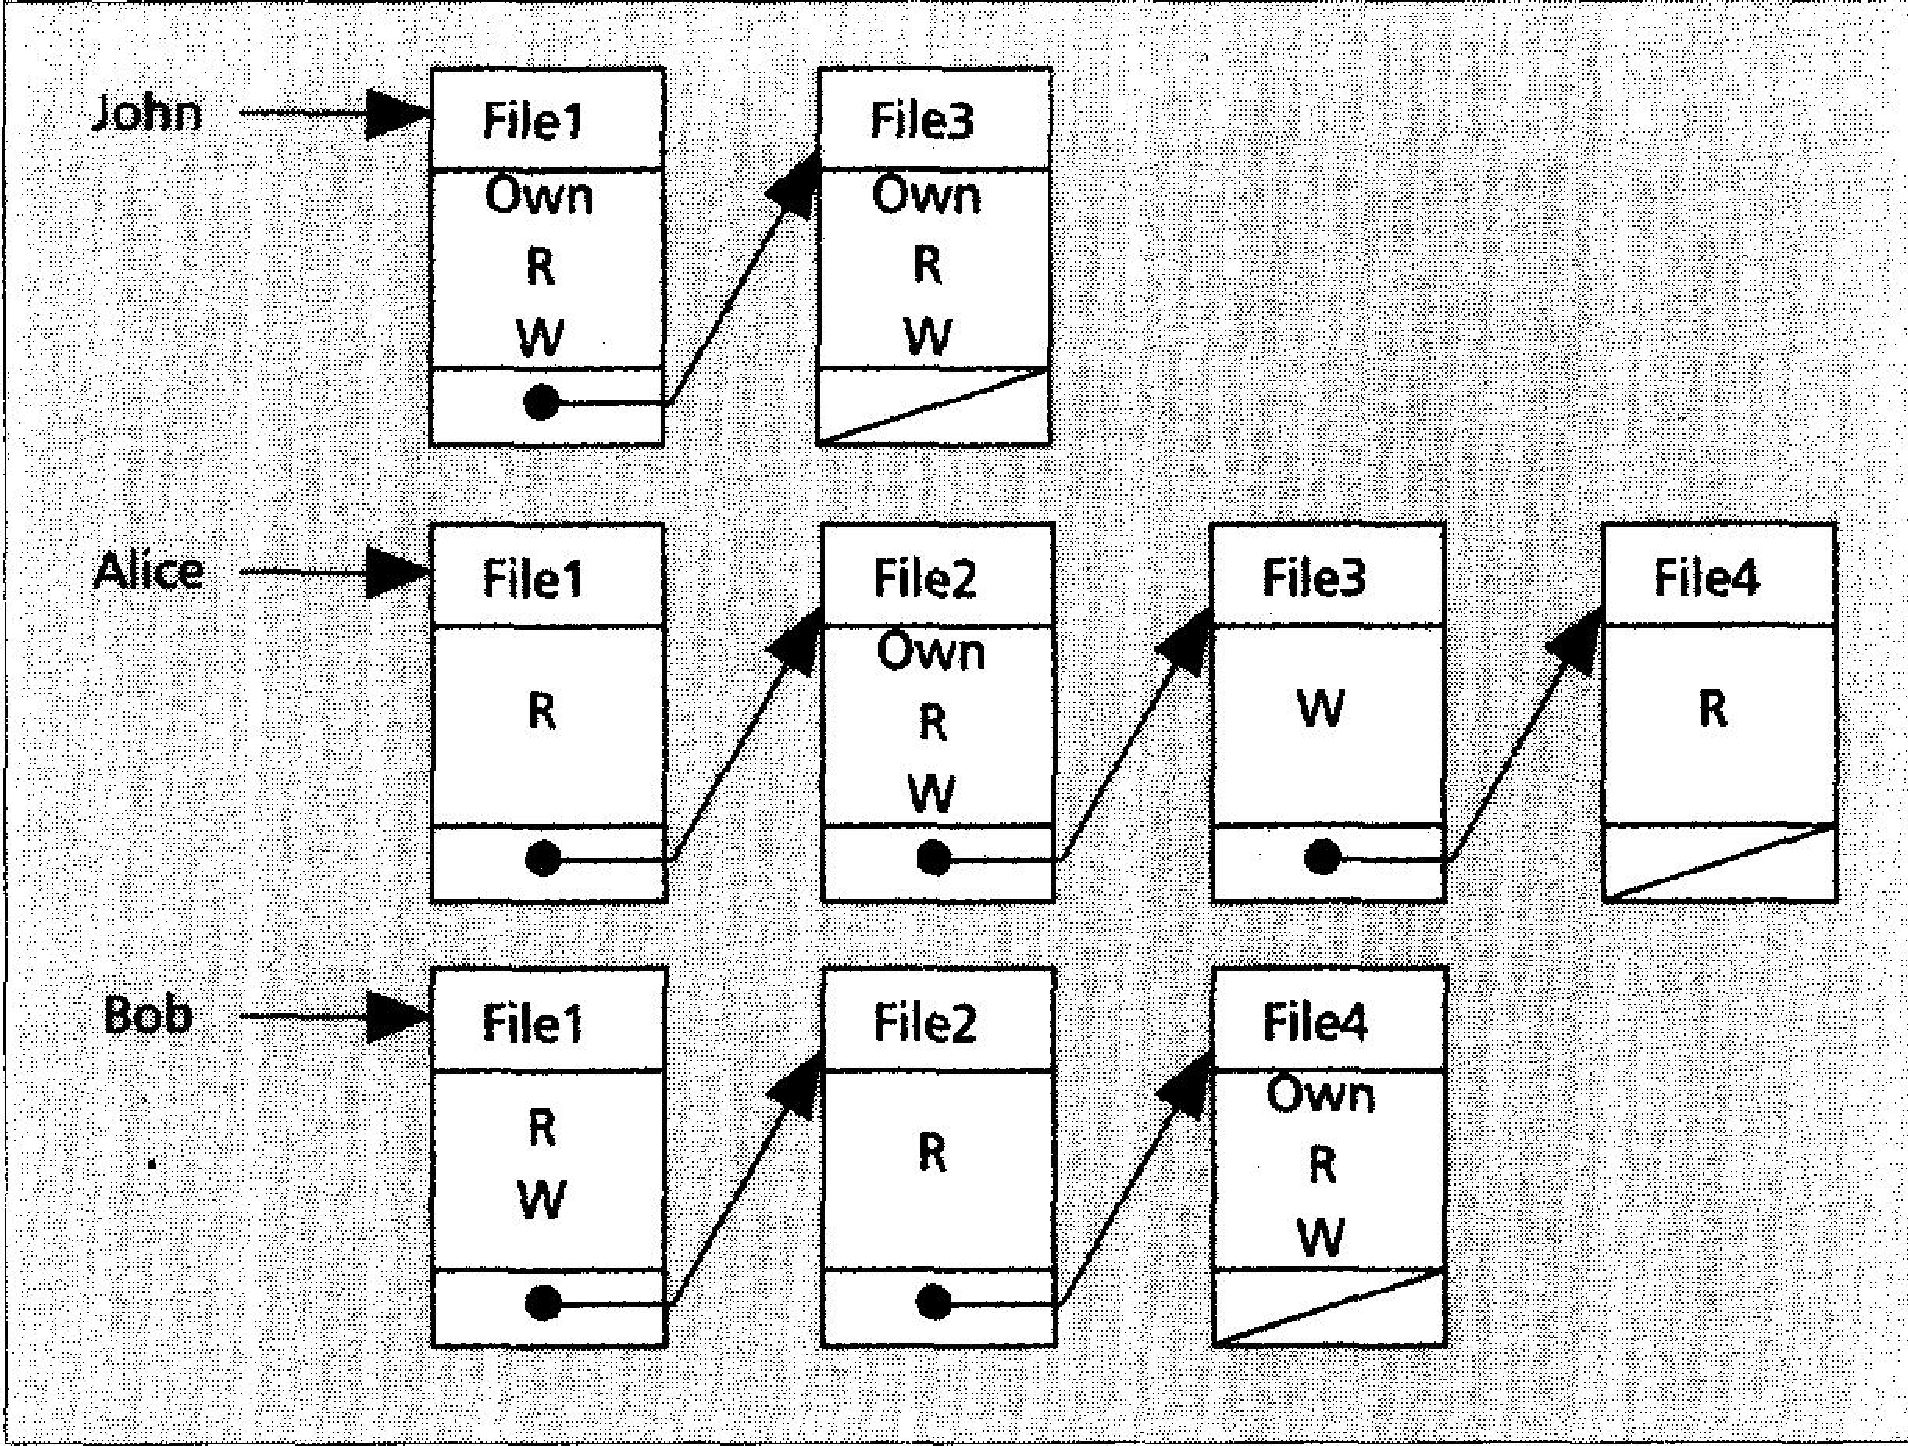
\includegraphics[height=2.5in,width=4in,angle=0]{capabilities.pdf}}
\caption{Capabiliy list for four files and three users.\cite{accessControlPrinciples}}
\label{fig:capabilities}
\end{figure}

\subsubsection{Hierarchical Cryptography for Access Control}
Hierarchical access control relies on different levels (or classes) of security which can be represented as labels in a partially ordered set (L, $≤$). These labels can be applied to users, $u$, and objects, $o$, using a many-to-many labelling function $lambda : U ∪ O → L$ where $U$ is a set of all users $u$ and $O$ is a set of all objects $o$. "$u$ is authorized to access $o$ if and only if $\lambda(u)≤\lambda(o)$\cite{mainPaper}."

\subsubsection{Interval-Based Access Control}
Interval-based access control works in a similar way to standard hierarchical access control however, unlike standard hierarchical access control, it is necessary to have a lower bound of access as well an upper bound. If $1, \dots , n$ is a totally ordered set of all possible security levels and $[x,y]$, where $1≤x≤y≤n$, is an interval associated with some user then that user can access an object $o$ associated with a security level $l$ where $1≤l≤n$ if and only if $l ∈ [x,y]$.
\newline \indent This idea can be extended to cover $k$-dimensional cardinalities:
\newline \indent ``Let $O$ be a set of protected objects, let $U$ be a set of users, and let $A_{1}, \dots , A_{k}$ be finite, totally ordered sets of cardinality $n_{1} , \dots , n_{k}$, respectively. We write $\mathcal{A}$ to denote $\prod_{i=1}^k A_{i} = A_{1} \times \dots \times A_{k}$.  
\newline \indent We say $[x_{i},y_{i}] ⊆ A_{i}$, where $1≤x_{i}≤y_{i}≤n_{i}$, is an \textit{interval} in $A_{i}$. We say that $\prod_{i=1}^k [x_{i},y_{i}] = [x_{1},y_{1}] \times \dots \times [x_{k},y_{k}] ⊆ \mathcal{A}$ is a \textit{hyperrectangle}. We write HRec($\mathcal{A}$) to denote the set of hyperrectangles in $\mathcal{A}$.
\newline \indent We assume that each object $o ∈ O$ is associated with a unique attribute tuple $(a_{1} , \dots , a_{k}) ∈ A$, and each user $u ∈ U$ is authorized for some hyperrectangle $\prod_{i=1}^k [x_{i},y_{i}] ∈$ HRec($\mathcal{A}$). Then we say that a user $u$ associated with $\prod_{i=1}^k [x_{i},y_{i}]$ is \textit{authorized} to read an object $o$ associated with tuple $(a1 , . . . , ak) ∈ \mathcal{A}$ if and only if $a_{i} ∈ [x_{i},y_{i}]$ for all $i$\cite{mainPaper}."
\newline \indent Some common implementations of this scheme are\cite{mainPaper}:
 \begin{itemize}
 \item \textit{Temporal} ($k=1$) where $\mathcal{A} = A_{1}$ and each integer in $1, \dots , n ∈ \mathcal{A}$ are in one-to-one correspondence with the time points. A 1-dimensional scheme follows the regular interval-based access control scheme as described above in which a user is associated with an interval $[x,y]$ and each object is associated with an integer. If the integer exists in the interval then the user should possess, or have the means to possess, the key to access the object.
 \newline \indent An example of this can be seen in Figure ~\ref{fig:hasse}. For instance if a user was associated with the interval [2,4] then she should be be able to derive the keys for the leaf nodes [2,2], [3,3] and [4,4] but should not be able to derive the key to access the leaf node [1,1].
 \item \textit{Geo-spatial} ($k=2$) where $\mathcal{A} = A_{1} \times A_{2}$. $\mathcal{A}$ represents a finite rectangular $m \times n$ grid of cells for which objects and keys are associated with a unique cell. Users are associated with an interval which correspond to a subrectangle of $\mathcal{A}$ where the user is able to derive keys for all cells in the area\cite{atallahGeo}.  More formally, ``each object is associated with
some point (x, y) and each user is associated with some rectangle $[x_{1} , y_{1} ] \times [x_{2} , y_{2} ] = (t_{1} , t_{2} ) : t_{1} ∈ [x_{1} , y_{1} ], t_{2} ∈ [x_{2} , y_{2} ]$.
We write $T_{m,n}$ (as an abbreviation of the more accurate $T_{m} \times T_{n}$) to denote the set of rectangles defined by a rectangular $m \times n$ grid of points: that is, $T_{m,n} \defeq [x_{1} , y_{1} ] \times [x_{2} , y_{2} ] : 1 ≤ x_{1} ≤ y_{1} ≤ m, 1≤x_{2}≤y_{2}≤n$"\cite{mainPaper}. Leaf nodes make up the $m \times n$ grid and are of the form $[x, x] \times [y, y]$ or $[x, y]$.
\newline \indent Two visualisations of this can be seen in Figure ~\ref{fig:geospatial}. Figure ~\ref{fig:geospatial}a displays $T_{2,2}$ as a "partially ordered set of subsets ordered by subset inclusion in which rectangles are represented by filled circles," while the second depicts $T_{2,2}$ where "nodes of the same color have the same area
(as rectangles): all rectangles of area 2 are filled in gray, whereas all rectangles of area 1 are filled white."\cite{mainPaper}
 \end{itemize}
 
\begin{figure}
\centerline{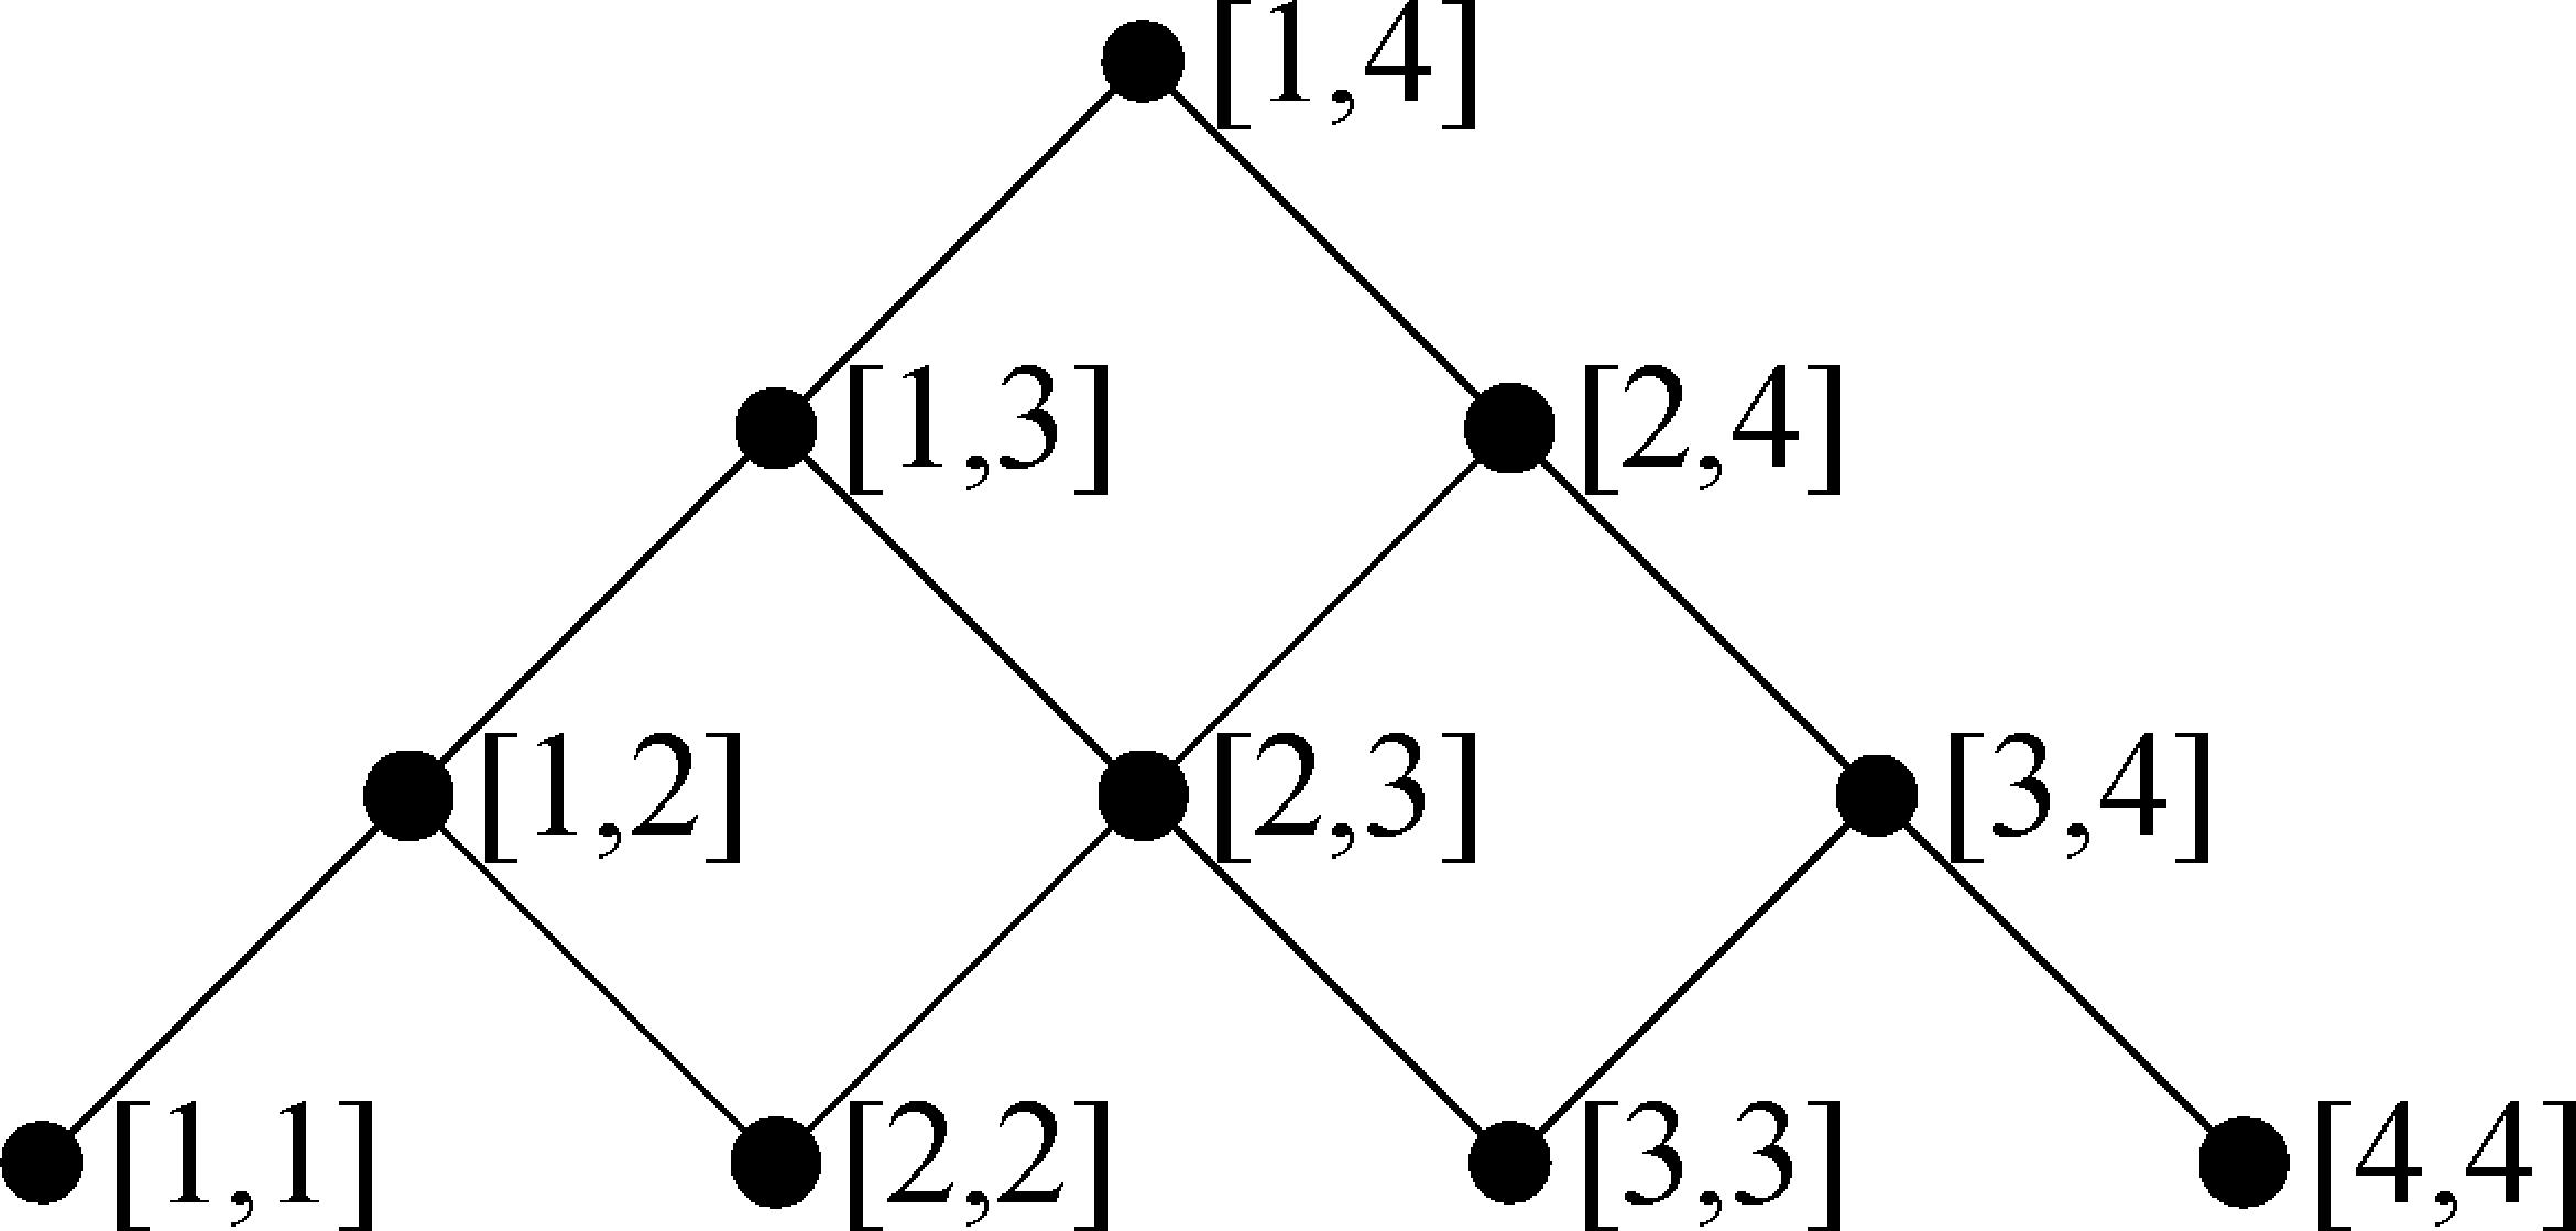
\includegraphics[height=1.0in,width=2in,angle=0]{hasse.pdf}}
\caption{The Hasse diagram of (T4 , $⊆$).\cite{mainPaper}}
\label{fig:hasse}
\end{figure}

\subsubsection{Key Assignment Schemes (KAS)}
A key assignment scheme (KAS) controls the information flow through the tree. The scheme dictates how a user is to derive access to objects she is permitted access to as well as preventing her access to objects she is forbidden from viewing. KAS are ``usually evaluated by the number of total keys the system must maintain, the number of keys each user receives, the size of public information, the time required to derive keys for access classes, and the work needed when the hierarchy or the set of users change.\cite{atallah2005}" As an example, the simplest possible KAS would be to assign every single key for which $k(y) : y<\le(u)$ where $u$ is a user and $le$ is a labelling function. This scheme, however, is not ideal and efforts are generally make to reduce the number of keys held by the user. To do this most schemes look to either provide additional public or private information. 
\newline \indent Recently a lot of work has been done in key assignment schemes, however not all of the proposed solutions are secure or efficient. As observed by Blanton[2007], the most efficient of the solutions achieve the following properties\cite{blanton2007}:
\begin{itemize}
\item Each node in the access graph has a single secret key associated with it.
\item The amount of public information for the key assignment scheme is asymptotically the same as that needed to represent the graph itself.
\item Key derivation involves only the usage of efficient cryptographic primitives such
as one-way hash functions.
\item Given a key for node $v$, the key derivation for its descendant node $w$ takes \textit{l} steps, where \textit{l} is the length of the path between $v$ and $w$.
\end{itemize}
 A few potential algorithms to test will be outlined here:
\begin{itemize}
\item \textbf{Iterative key encrypting (IKE)} - For each edge in the graph the child key is encrypted with the parent key and published as public information. The user is then, using a single private key, able to iteratively derive any child key using that information\cite{lazyEncryption}. The AFB scheme by Atallah et al. is an example of this KAS, offering\cite{atallah2005}:
\begin{itemize}
\item A single private key held by the user
\item Permits only a hash functions to derive keys
\item Derivation of a descendant node's key requires $\mathcal{O}(l)$ operations where $l$ is the length of the path between the nodes
\item "Updates [i.e., revocations and additions] are handled locally and do not propagate to descendants or ancestors of the affected part of G"
\item "The space complexity of the public information is the same as that of
storing [the] graph."
\item Provably secure against collusion
\end{itemize}


\item \textbf{The Akl-Taylor scheme} - Created by Akl and Taylor, this node-based scheme is the first KAS created. Key derivation in a node-based scheme eliminates the need for recursive calculations, instead the algorithm works as follows\cite{lazyEncryption}:
\begin{itemize}
\item The RSA key generator is called to obtain $(n, e, d)$, of which only n is used
\item $s$ is chosen at random from $\mathbb{Z}^{*}_{n}$
\item A mapping is chosen $\phi \rightarrow \mathbb{N}^{*}$ such that $\phi(x) | \phi(y)$ if and only if $y≤x$.
\item The key for $x$, $k(x)$, is defined to be $k(x) = s^{ \phi (x)} \bmod n$.
\item ${n} \cup (\phi(x) : x ∈ L)$ is published publically.
\end{itemize}
where ``$(n, e, d)$ such that: $n = pq$, where $p$ and $q$ are distinct odd primes; $e ∈ \mathbb{Z}^{*}_{\phi(n)}$, where $\phi(n) = (p − 1)(q − 1)$, $e > 1$, and $(e, \phi(n)) = 1$; $d ∈ \mathbb{Z}^{*}_{\phi(n)}$, where $ed \equiv 1 \bmod \phi(n)$."
\newline Using private key $k(x)$ to derive $k(y)$ where $y≤x$ the following formula is used:
\begin{align*}
(k(x))^{\frac{\phi(y)}{\phi(x)}} = (s^{\phi(x)})^{\frac{\phi(y)}{\phi(x)}} = s^{\phi(y)} = k(y).
\end{align*}
where $\phi(x)$ and $\phi(y)$ is publically available information.
\newline \indent This scheme while secure (when $\phi$ is chosen appropriately) and fast, requires a lot of public information.
\end{itemize}
Some KASs for special case scenarios exist, such as for when the number of leaf classes is substantially larger than the number of non-leaf classes.\cite{largeLeaf} There has also recently been a number of works on elliptic curve cryptography (ECC)\cite{ecc1}\cite{ecc2}, however this method relies on public-key cryptography and this project will initially focus on symmetric key techniques.

\begin{figure}
\centerline{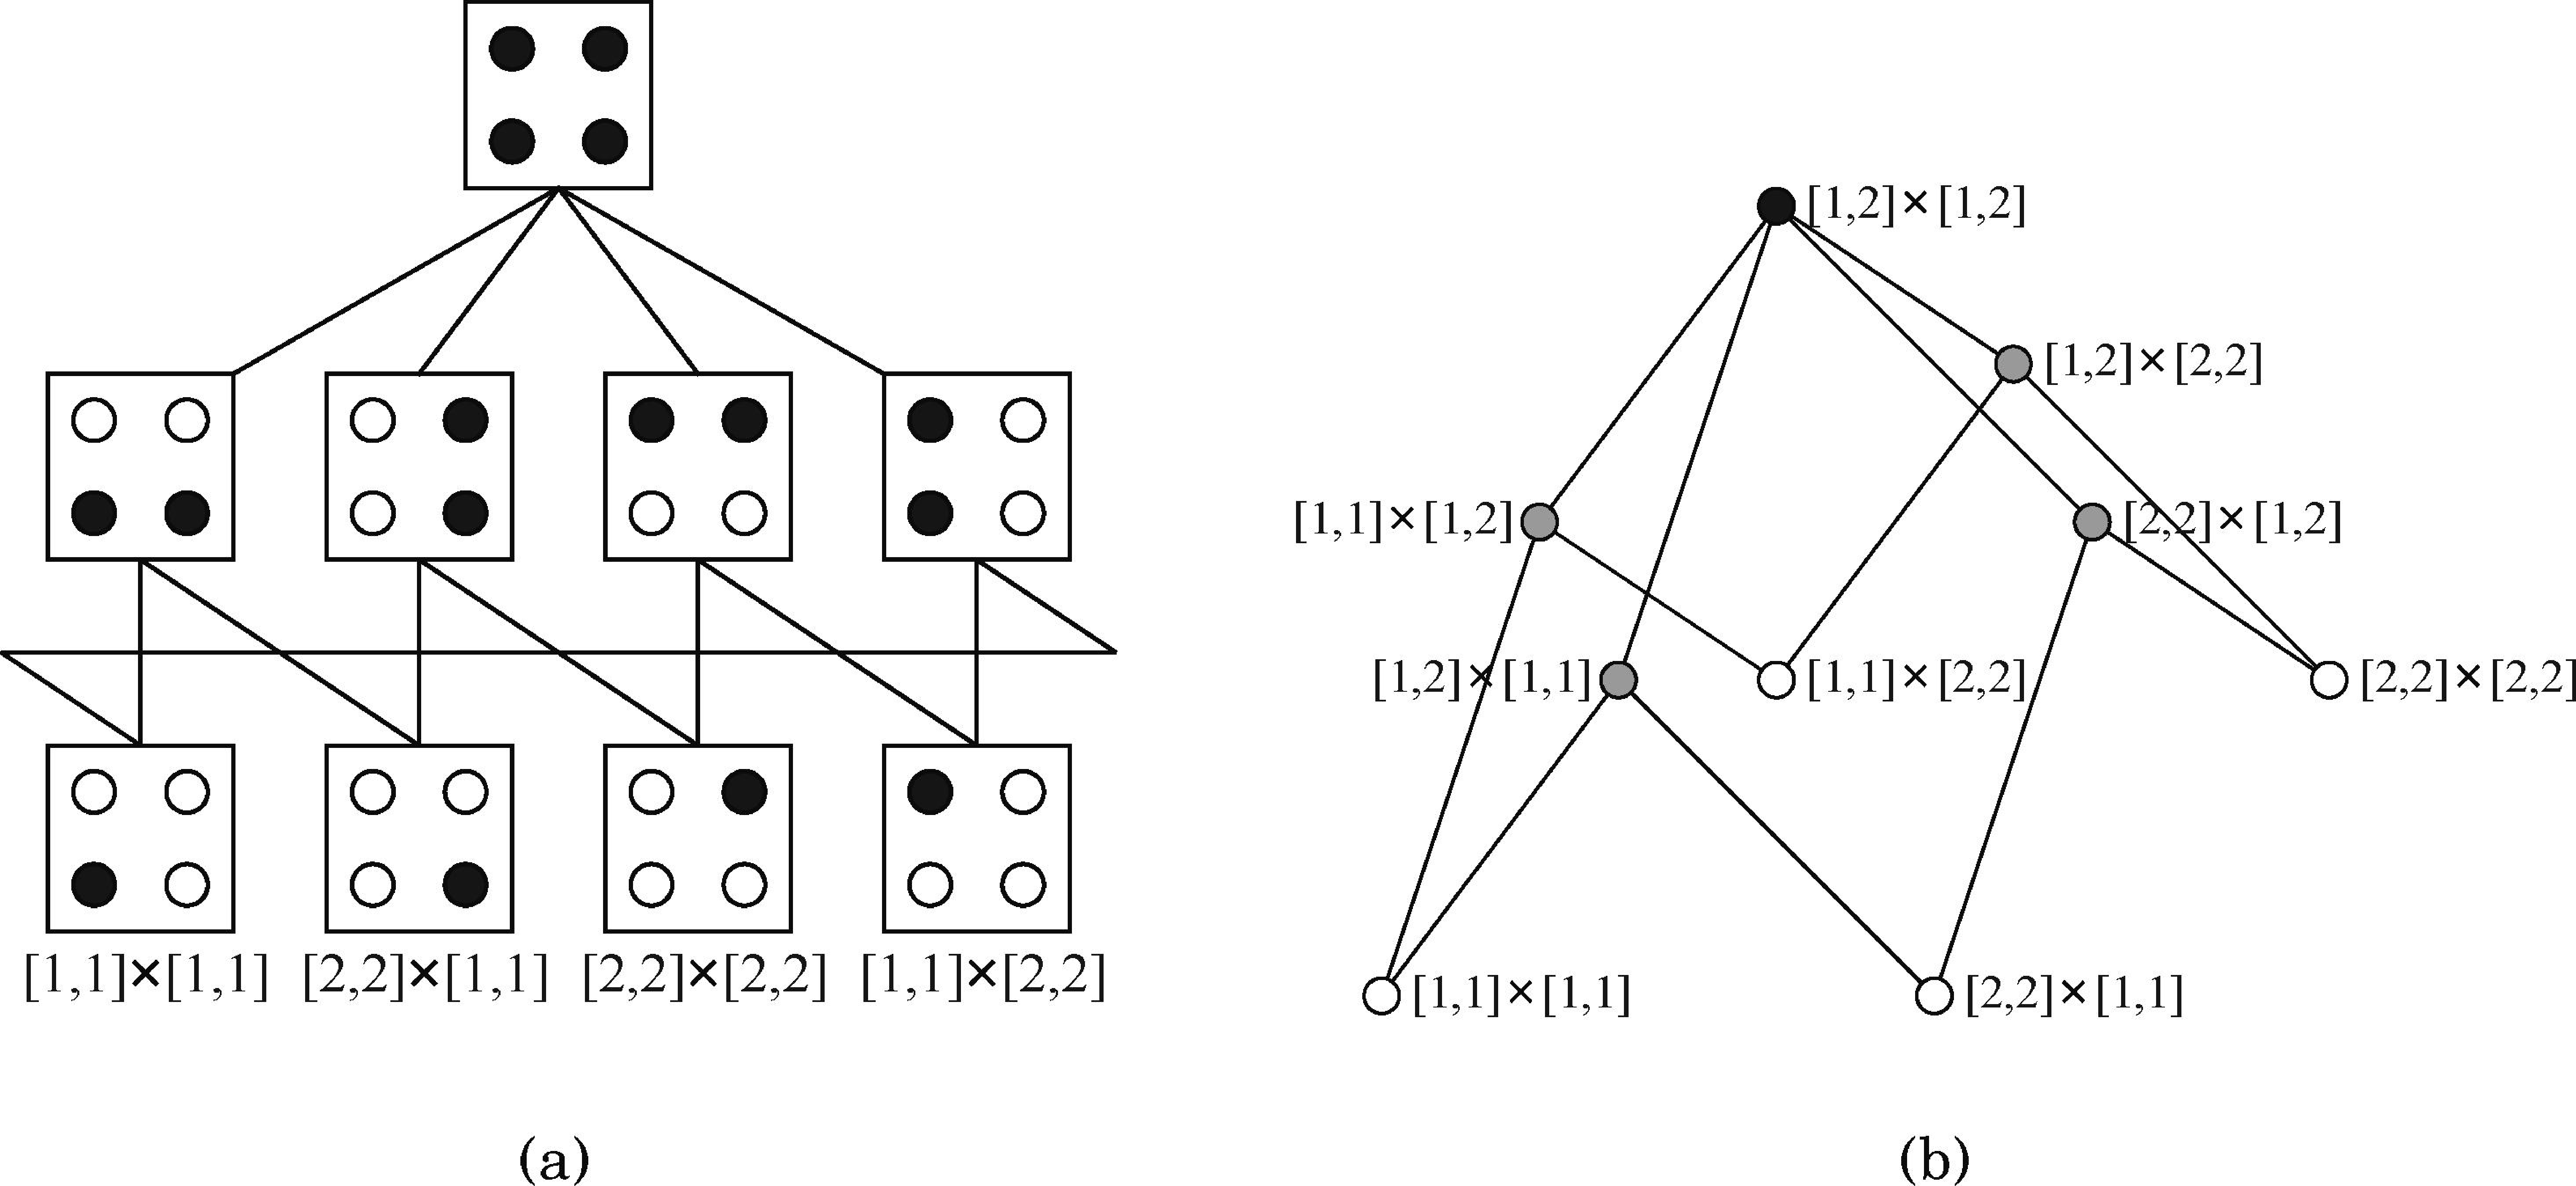
\includegraphics[height=3.0in,width=6in,angle=0]{geospatial.pdf}}
\caption{Two representations of $T_{2} \times T_{2}$.\cite{mainPaper}}
\label{fig:geospatial}
\end{figure}

\subsubsection{Revokation of Permissions and Re-encryption}
There are occasions where a user previously granted access at some security interval is later revoked of those permissions. If the user was associated with a security label $l$ then the revoked user has held a key which grants her access to objects at every node within her security interval, $l' \le l$. Due to this it is no longer acceptable to continue using the same key for any $l'$ as the revoked user would be able to view or edit future and existing objects that she should no longer have access to. Thus for every $l'$ it is necessary to replace the key associated with the label with a new key with which every object associated with $l'$ is re-encrypted with.
\newline \indent The most obvious way to achieve re-encryption is to immediately re-encrypt every object associated with every $l'$ the moment the user has been revoked and distribute the new keys to the appropriate users to replace the old key. This method ensures the revoked user has no access the objects she previously had access to, therefore providing robust security, and the users who have not had their permissions revoked continue as normal with the new key. However the number of objects associated with $l'$ may well be extremely large meaning that re-encrypting all of them instantly could take a long time, possibly disrupting the service. It also may well be the case that a significant number of the objects may not be viewed or edited for some time, if ever. An alternative to this method is \textit{lazy re-encryption}.
\newline \indent Lazy re-encryption does not instantly re-encrypt all objects, instead an object is re-encrypted with the newly assigned key for the security label $l'$ only when it is edited for the first time after the revokation by any user. The result is that the workload of re-encryption is spread out over time and is only performed when absolutely necessary. Employing lazy re-encryption requires the user to possess more than one key - one key for objects yet to be encrypted and one for objects encrypted with the new key.\cite{lazyEncryption} This means that the revoked user has the capacity to view objects while they remain unchanged and not yet re-encrypted. While logic suggests that the user who has been revoked has already been able to see the object during the time their permissions were valid meaning that it is unlikely to pose a real threat, this may not be acceptable in every scenario. To avoid this problem another solution may be to, instead of waiting for the object to be edited, wait for the object to be requested for a read. This way the user will need to possess the newly assigned key to read the object however the burden of re-encryption is still spread out over time. It can also be noted that if there are a number of users revoked over time and there are sporadic reads/writes of different files there will be a large number of keys being used for files associated with the same security level that a single user is required to hold. To keep the number of keys down it may be desirable at times to re-encrypt objects even when they are yet to be accessed.

\begin{figure}
\centerline{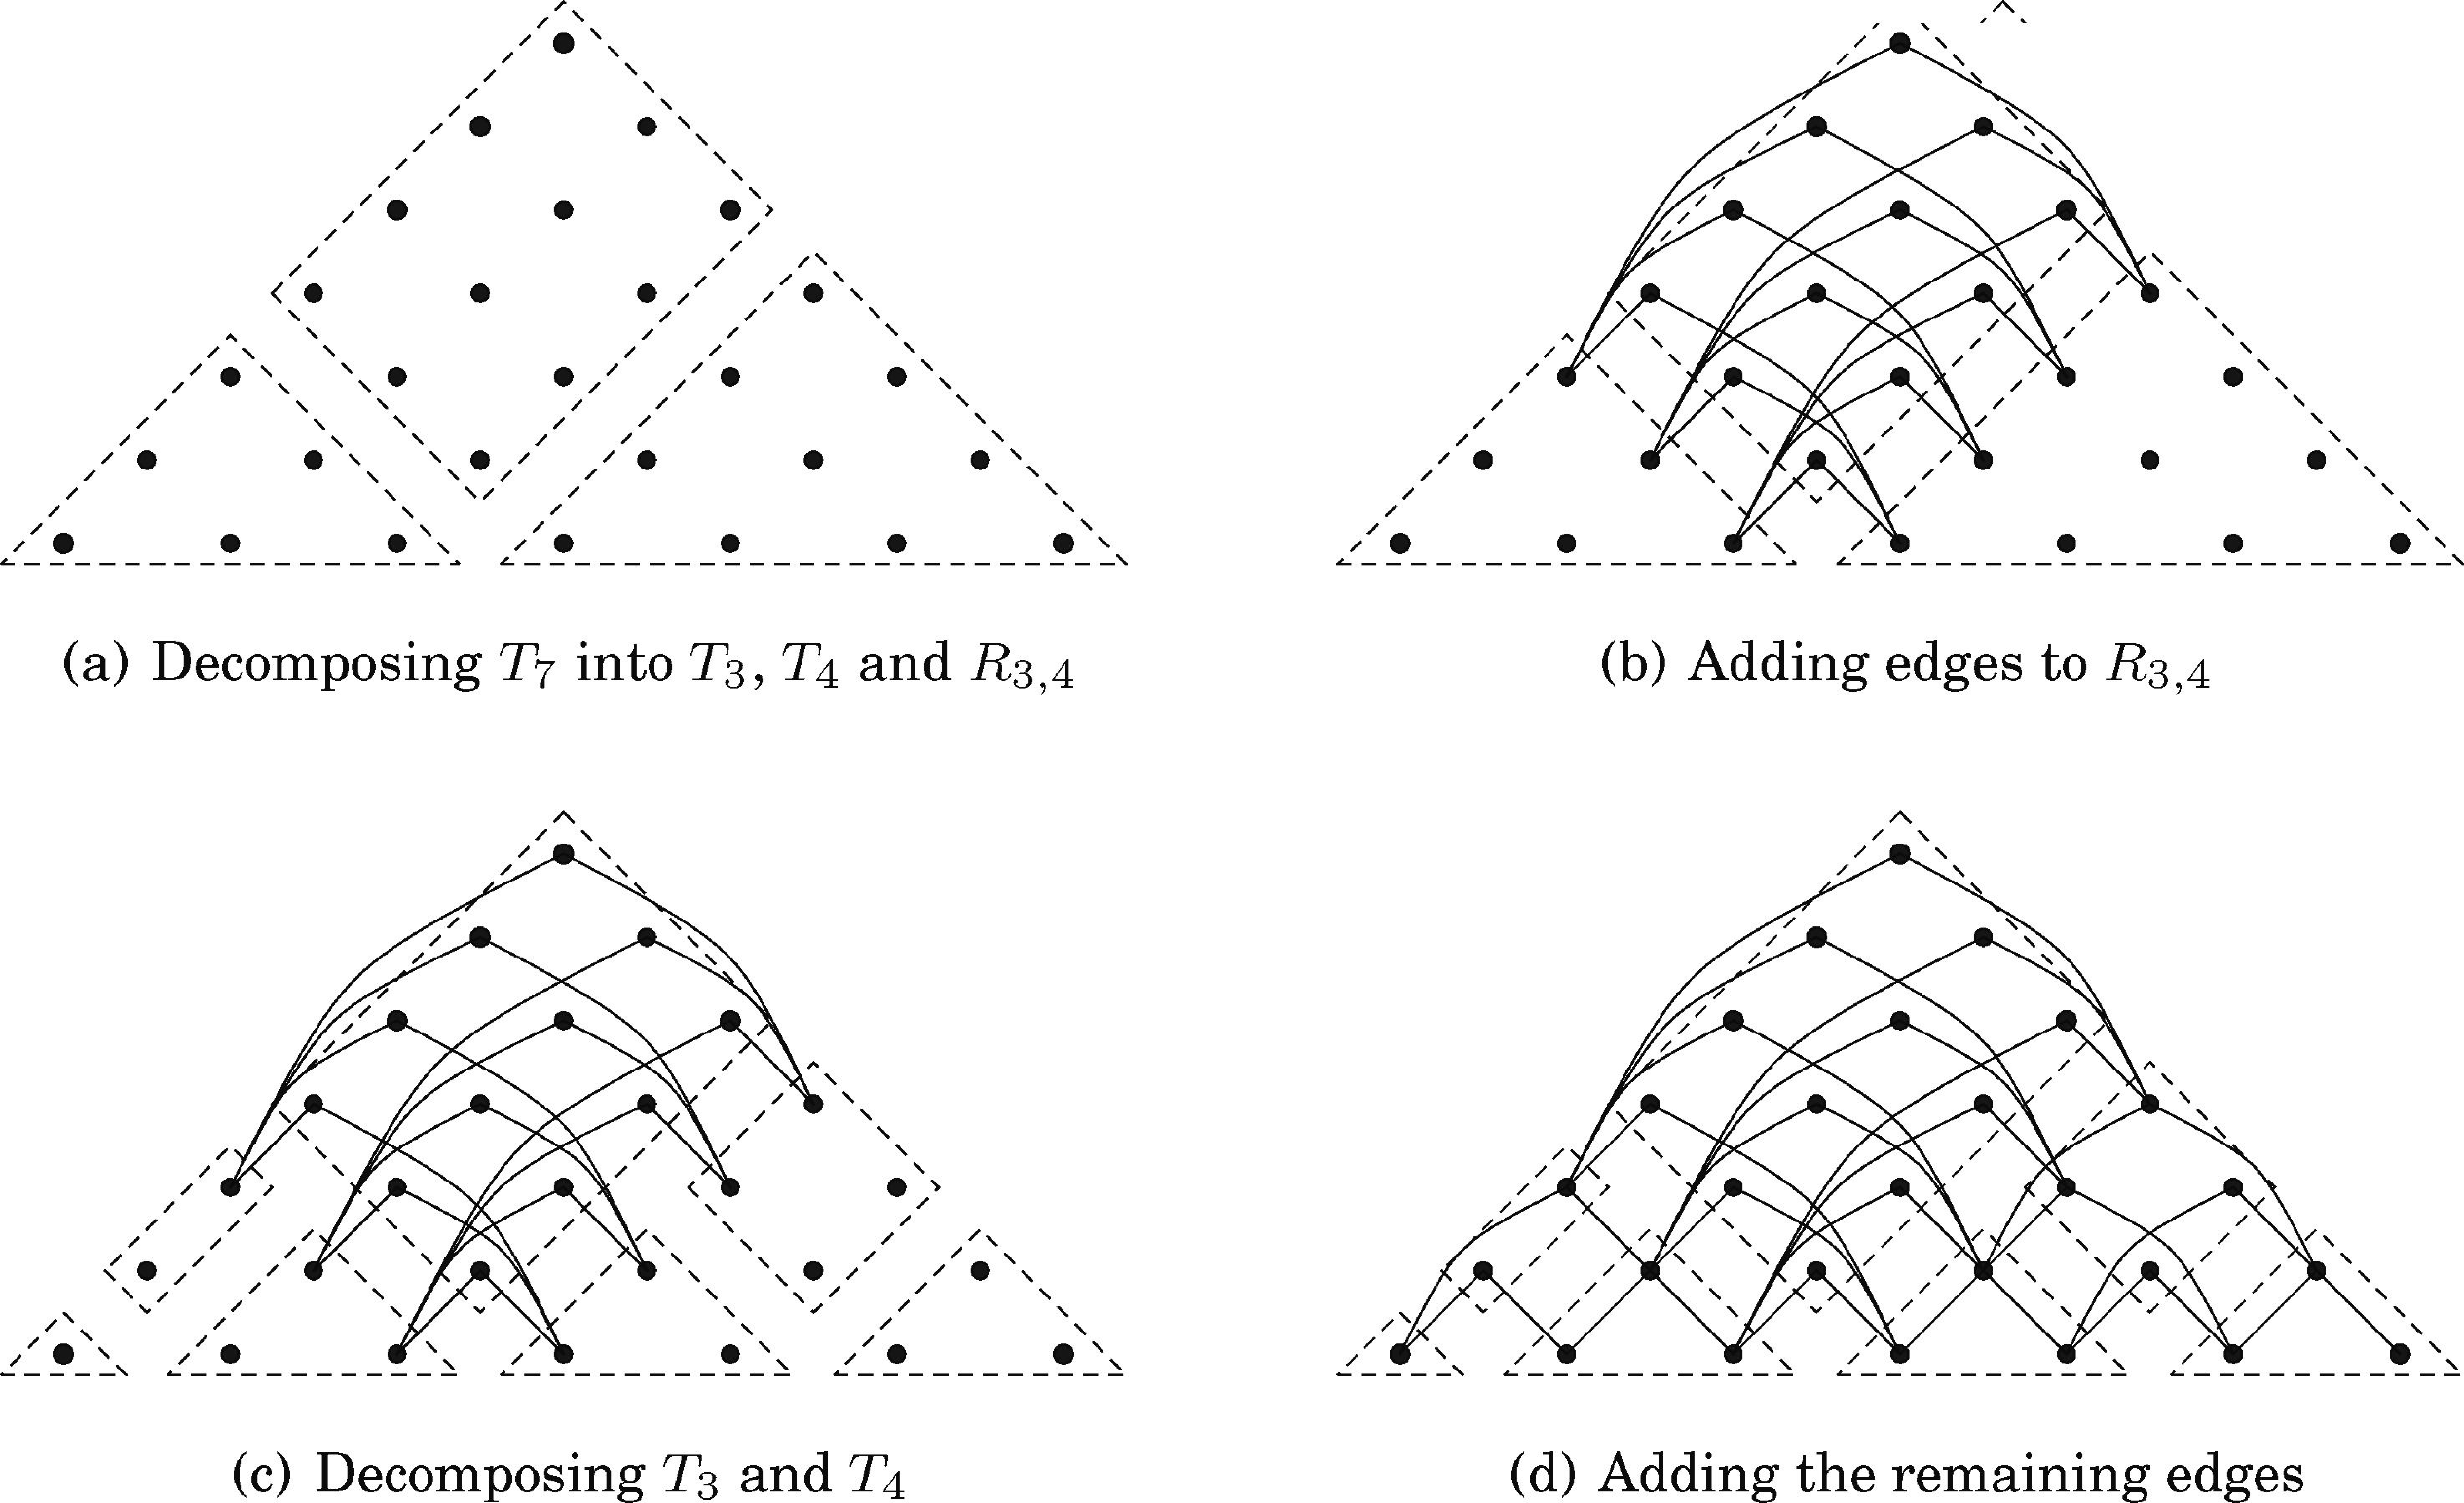
\includegraphics[height=3.0in,width=6in,angle=0]{binarydecompo.pdf}}
\caption{The binary decomposition of $T_{7}$.\cite{mainPaper}}
\label{fig:binarydecomp}
\end{figure}

\subsubsection{Building the Tree}
Crampton[2011]\cite{mainPaper} describes a process of binary decomposition which uses recursive labelling methods to separate the whole tree into nodes. In general the result is a smaller tree with some unnecessary edges being removed meaning that key derivation takes less time and the required storage space for the tree is smaller. The following describes how the process works:
\newline \indent If $T_{m}$ represents the set of intervals where $m$ is the cardinality then ``let $l = \lfloor m/2 \rfloor$ and $r = \lceil m/2 \rceil$. Now $T_{m}$ comprises:
\begin{itemize}
\item A copy of $T_{l}$, containing the minimal elements $[1, 1], \dots , [l,l]$.
\item A copy of $T_{r}$, containing the minimal elements $[l + 1, l + 1], \dots , [m, m]$.
\item A copy of rectangle $R_{l,r}$, containing the remaining nodes in $T_{m}$."
\end{itemize}
The result of this procedure can be seen in Figure ~\ref{fig:binarydecomp}a for $T_{7}$.
\newline The next step is to begin adding edges. An edge is added from every node in $R_{l,r}$ to two other nodes, a single node in $T_{l}$ and a single node in $T_{r}$. ``In particular, for node $[x, y]$ such that $x<l≤y$, we add edges from $[x, y]$ to $[x, l]$ and from $[x, y]$ to $[l + 1, y]$."
\newline This algorithm is then recursively applied to $T_{l}$ and $T_{r}$ until $l, r ≤ 1$. The final result of this process can be seen in Figure ~\ref{fig:binarydecomp}d.
\newline \indent It is clear to see that the information flow policy is still upheld, ie. each node still has access to all other nodes it previously had access to before the binary decomposition however it has not gained access to any new nodes.
\newline \indent Crampton details how this algorithm can be extended to temporal, geo-spatial and general interval access control.

\subsection{Related work}
To the best of my knowledge no current commercial software implements hierarchichal cryptography for use in file sharing.
\newline \indent Established file sharing platforms such as Dropbox and Mega offer users a way to share their files with other users. This can be in the form of a single file or an entire folder. Our system could be simulated using the folder sharing, where each folder represents a security level and the folders are simply shared folders with the desired users one-by-one. Of course, this method requires a lot more work.
\newline \indent Existing military based models such as the \textit{Bell-LaPadula model} (BLP) could be applied to create a similar environment to which we are attempting. Using BLP works by labelling each object (file) and user with a security level, such as `Unclassified' ... `Top Secret'. BLP prevents subjects from reading objects with a higher level and from writing to objects with a lower level. We could attempt to use this by assigning each user their own BLP and give them full control of labelling. However the military environment is stricter than our target environment and we are left with the unnecessary and unwanted write restriction and no method of sharing the files outside of the network the model is located is specified.

\section{Initial Assessments}

\subsection{System design}
In this section we will dicuss the required components of the system, why they are necessary for our system and how we shall go about achieving each one. The required components of the system are:
\begin{itemize}
	\item \textbf{Information storage}
	\item \textbf{Authentication}
	\item \textbf{Encryption of files}
	\item \textbf{Key exchange}
	\item \textbf{Friends}
	\item \textbf{Key revocation}
	\item \textbf{Version control}
	\item \textbf{GUI}
\end{itemize}

\subsubsection{Information storage}
We need a method of keeping track of the information associated with the files uploaded, such as the security level, initialisation vector, the user who uploaded it, as well as information about each user, such as authentication details and friends. We need to keep track of this information to be able to display it back to the user and ensure only authorised operations are carried out by authorised users.
\newline \indent The traditional way of achieving this is to allocate a single authority who keeps track of a database. In this model a user is required to communicate with the authority to conduct actions who then verifies that the action is permitted. When an action has been verified for this user the authority may send some information required for the action to process and on completion of the action the user may send the necessary information to the authority to store for latter use. The most popular way of achieving this is using the \textit{Client–server model}. Using the Client–server model each entity is modelled by either a client or a server. In our environment each user is modelled by a client and our single authority is modelled by a server. However, there are issues involved in using a centralised authority. Having a single server which is not able to process all of the traffic from the clients introduces a bottle neck. There are also privacy issues involved by housing information in a centralised authority. The user must trust that those who control the information do not have malicious intent and are competent enough to protect the information sufficiently or are simply unlucky enough to fall victim to a `unpreventable' attack.  
\newline \indent It is possible to keep track of the information we need in a manner which does not require a centralised authority. We could attempt to implement a peer-to-peer network similar to that used by Bitcoin today, that is to allow each user to submit updated friends lists and file information (ie. unique file identifier and associated security level) into a public record. However implementing such a system requires a large number of users to donate a large amount of processing power to authorise is submission by users. While Bitcoin can encourage this with financial rewards we can offer no such thing. This model also requires each users friend list, including each user and their associated security level, to be public as well as the number of files each user has submitted at which security level.
\newline \indent Due to the the Client–server model being well established, familiar with many users and the easier option to implement that is what we shall use for this system.

\subsubsection{Authentication}
As we are using a Client–server model we need some way for the client to authenticate themselves with the server. The traditional manner of achieving this for each user to have a unique, public indentifier, a username, and private information for the client to verify who they say they are, a password. Upon log in the client must provide both pieces of information to the server before being authorised to perform operations unique to that user as well being provided information unique to that user.
\newline \indent In order for the server to be able to verify that the username and password that the client supplies are indeed correct both need to have been stored previously for the server to retrieve. Due to the username being public there are no privacy issues in storing it as plaintext in the database. The password is private information and so care must be taken before it is stored, due to privacy issues as well as security ones if the database is compromised. This problem can be solved by using a password hasher before the password is stored in the database. Doing so means that the plaintext password can not be read by database administrators and if the database is compromised an attacker can not simply resubmit the hashed password and gain access to a user's account. The hashing must take place on the server side - this is because, while the user's plaintext password can not be read, in the event of the database being compromised the hashed password can be simply re-sent to the server and any security benefits of hashing the password would be lost. Care still needs to be taken in sending the plaintext password to the server. In order to prevent eavesdropping we will simply securely send the plaintext password securely, either through a secure channel such as a HTTPS tunnel or encrypted with a public key belonging to the server.
\newline \indent In summary, we shall hash the passwords which are sent to the server securely, serverside and then store the hash in the database which can the be used for authentication given a username and plaintext password.

\subsubsection{Encryption of files}
In order for our users to safely upload our files into a `public' domain they need to encrypt the files. In our scenario the same authority on the file is the  only person who we wish to grant access to the file (until it is shared, which we shall address in the \textit{Key exchange} section.) For this we shall use symmetric key cryptography. While we could use public key cryptography to achieve this symmetric key cryptography is faster and, as we have no prior knowledge on the size of the files the user may wish to upload, this speed difference may well be significant.

\subsubsection{Key exchange}
Given a key a user will be able to derive any key with a security level below that for a given user. However assuming that a user wishes to grant another user access to a maximum of some level the key for that level needs to transferred to the other user for without any other user being able to observe it. This is the type of scenario which public key cryptography was designed. In order to achieve this behaviour using public key cryptography, each user can generate their own public and private key pair and send the public key only the server to be stored publicly. When a user wishes to share their files with another user they can then request the public key of the user in question and then encrypt the symmetric of the highest level they wish to share at then send that to the server for storage. The receiving user can decrypt the key using their private key which they have stored.

\subsubsection{Friends}
There are a few options available to us in how we handle the adding of friends. We could allow for either the owner of files to request to share the files with another user or for a users to request access to another user's files. There are no real positives or negatives associated with either method but it makes more sense for the owner of the files to decide who has access, rather than rely on the correct people to request access.
\newline \indent When the owner of files decides another user is entitled to access some of them we shall post a request to that using stating the owner whishes to share files with them. The reason for this is that without requests the user may be subject to un-wanted or potentially malicious files which they would have no way of preventing. It may also be the case that the underlying network charges for the amount of space used and the users may wish to be selective on who can share files with them.
\newline \indent As all of the files are encrypted, when a user is granted access to some owners files at some level we have the option on which files we share with them. Of course the files they have been granted access to should be be shared with them, however we could simply share all of the files the owner has uploaded with them. This is acceptable as the user is only able to decrypt ones for which they have been able to derive keys for. The benefit of this method is if in the future the user's access level is increased by the owner no further change is needed in regards to the files shared with them. The downside is the user can see the file names of the files they do not have access to, all files uploaded in the future by the owner which they do not have access to has to be shared with them and unnecessary space is taken by files the user is not interested in. For this reason we shall only share the owner's files for which the user has access to.
In summary, in our system an owner of files will be able to request to share their files with a users at some level. With the request shall be the symmetric key representing the highest level the user wishes to share with the potential friend. The key shall be encrypted with the potential friend's public key. If the potential friend accepts the request, while all uploaded files are considered to be in the public domain, we will only share files directly to the new friend for which they will be able to decrypt (ie. if the levels available are 1-5 and this users is permitted for levels <= 3 then we shall share files labelled <= 3 but not > 3.)

\subsubsection{Key revocation}
There may come a point when a user no longer wishes for a friend to be able to access their files. We are able to implement this feature in one of two ways, as previously describe - immediate or lazy. The computational requirement for both is the same, however lazy key revocation spreads the computation needed over time. Lazy key revocation requires much more complex logic and so due to the time constraints on this project we shall implement immediate key revocation. 

\subsubsection{Key storage}
As discussed in the previous sections, \textit{Encryption of files} and \textit{Key exchange}, each user is required to store some number of symmetric keys and a single private key. The privacy of these keys is fundamental to the functioning of the system in the way we desire. If the symmetric keys are compromised then all of the user's files can be accessed at will as well as all of the keys which have been shared with this user. If the private key is compromised then all future keys shared with this user can be intercepted and derived. Due to these reasons the keys need to be carefully stored. To avoid storing the keys in unprotected files there are software implementations to keep them in called \textit{key stores}. These key stores can be protected by a password which has to be supplied before the keys can be accessed. It would be more secure if we require a user to supply two seperate, distinct passwords. One password is sent to the server to be hashed as previously explained and the other is not sent to the server and instead used to create a key store. This means that even in the event of the database at the server being compromised the attacker is still unable to access the user's key store even with access to user's particular machine. However this method requires the user to remember two different passwords and could be consider an unreasonable request for the events in which it would provide any extra security. In the case where the likely attackers are known personally to a user, such as in the same company or in the same household, it likely be a significant improvement in security. As we do not have any real knowledge on our likely userbase's situations we shall simply reuse the password for server authentication as the password for the key store.

\subsubsection{Version control}
It may be desirable for the users who receive shared files to be able to edit them and update the file owner's version of the file. This would prevent the user who changed the file from having to upload the file themselves and integrate file management into their own security levels - for instance they may not wish for that user to see any of their files which they would be required to do if they uploaded changed file at some security level and shared that level's corresponding key with the owner. Allowing people to update the file at other user's locations circumvents the need for this.
\newline \indent However an issue arises when two users the file owner has shared the file with are editing the the the file concurrently. If one user updates the version of the file and then the other updates it soon after the first update will be lost in the public domain. Unfortunately it is outside the scope of this work to deal with such issues in a meaningful way. One measure we can take in an attempt to prevent this is to ripple out the changes to all users who have access to the file. As users are required to download and decrypt the file to a seperate location this would not overwrite the changes any user may make but it will alert each user that changes have been made which may wish to incorporate into their own changes before the version themselves.
\newline \indent It can not be assumed that this behaviour is desired for every friend added. We will add an option when a user adds a friend whether that friend is permitted to update files. This option, in a sense, is similar to granting read access or read and write access. This would work by friend privileges being stored in the database and when the friend desires to update the file they are required to verify with the server before the action is permitted.

\subsubsection{GUI}
While the system we are designing is perfectly usable in a command line window, the tables of data, such as list of the user's own files, friends and files shared with them, would far easier to display in visual tables. The multitude of actions they are able to perform with the data would also be accessed more easily in a graphical for mrather than a text based form. It is also possible that retaining the the system in a command line window would reduce the potential user base a great deal. For these reasons we shall design a simple interface with which to view and manipulate the files and friends.


\subsection{Algorithm choices}
In this section we shall decide which algorithms we shall use to perform the tasks described in the previous section and attempt to rationalise each decision.
\newline \indent There are 4 key decisions to be made when choosing to employ a Crytographic algorithm. These are:
\begin{itemize}
	\item \textbf{Algorithm} - The algorithm itself
	\item \textbf{Mode} - The mode of operation used
	\item \textbf{Key size} - The size of the key used for encryption and decryption
	\item \textbf{Padding scheme} - The method to increase the size of the file to be encrypted in order to force into a multiple of the block size of that algorithm.
\end{itemize}
Here we will discuss which algorithms to use for this project and why.

\subsubsection{Symmetric Algorithm}
\begin{itemize}
	\item \textbf{DES} - A block cipher which used to be government standard. DES uses 56bit keys, however such small key lengths have proven to be insecure (eg. by the `EFF DES cracker') and can no longer be used safely.
	\item \textbf{3DES} - A variant on DES in which plaintext is fed through 3 seperate instances of DES using up to 3 different keys. 3DES, with 3 unique keys, is secure up to $2^112$bits of security, which is very secure. However DES is designed for hardware implementations and so it is slow when used in software which, unfortunately, is what we wish to use it for.
	\item \textbf{Blowfish} - 64 bit block size with up to 448 bit keys.
	\item \textbf{Twofish} - Successor to Blowfish. 128-bit block size with up to 256-bit keys
	\item \textbf{AES} - Uses 128-bit blocks with up to 256-bit keys. The current government standard.
\end{itemize}

AES is by far the most popular block cipher in use today and is currently approved by FIPS for use.\cite{aesFIPSApproved}
There is no reason not to use AES and so that is what we shall use.
\\
\\
AES supports the following modes of operation:\cite{aesModes}
\begin{itemize}
	\item \textbf{ECB} - Has been shown to be vulnerable if it used to encrypt more than one block of data with the same key. In our case, it can not be used to encrypt a file larger than 128-bits. ECB also has the undesirable trait where each plaintext block encrypted with the same key results in the same ciphertext block. This is undesirable as attackers are able to detect trends in an individuals encryptions. Requires padding.
	\item \textbf{CBC} - Each plaintext block is XORed with the previous block before it is encrypted by block cipher. An initialisation vector (IV) is used to XOR the first block. The ciphertext generated from the plaintext will different each time iff the IV is different. Requires padding.
	\item \textbf{CFB} - Requires padding
	\item \textbf{OFB} - Turns the block cipher into a stream. Does not require padding.
	\item \textbf{CTR} - Similarly to OFB, CTR turns the block into a stream cipher. Does not require padding.
	\item \textbf{EAX} - A variation on CTR which includes integrity checks
	\item \textbf{GCM} - A variation on CTR which includes integrity checks
\end{itemize}
While it is true that the modes that require padding, such as ECB, CBC and CFB can be subject to padding oracle attacks, in our implementation we will have no such oracle and so we need not worry about such attacks.\cite{oraclePadding}
\newline We will use CBC for no reason other than it is widely supported and relatively simple to implement while not sacrificing any security if implemented correctly.
\\
\\
AES supports the following key sizes:
\begin{itemize}
	\item \textbf{128-bit}
	\item \textbf{192-bit}
	\item \textbf{256-bit}
\end{itemize}
The only weakness possible resulting from the size of the key chosen is that of brute force attacks. A 128-bit AES key provides 128-bits of security (pg. 64, Table 2) and is speculated to be safe beyond the year 2031 (pg. 67, Table 4).\cite{nistKeys}
While we may choose to use a 256-bit key `just to be safe' it is unlikely that this system will be around in 30 or 40 years and so this sort of precaution is unnecessary. Using a 192-bit key instead would cause us to take a performance hit of around 20\% while a 256-bit key would cause a 40\% hit, due to the fact that 128-bit, 192-bit and 256-bit keys require 10, 12, 14 rounds respectively (pg. 14, Figure 4)\cite{announcingAES}. Due to this, using a smaller key is desirable for performance.
\newline For these reasons we shall use a 128-bit key for AES in our system.



\subsubsection{Asymmetric algorithm}
As we wish to use asymmetric encryption for key exchange the options available to use are:
\begin{itemize}
	\item \textbf{RSA} - Relies on the difficulty of factoring large primes
	\item \textbf{ElGamal} - Relies on the difficulty of solving the discrete logarithm problem.
	\item \textbf{DSA} - A variant on ELGamal used for the digital signatures
	\item \textbf{Diffie-Hellman} - A method of key exchanged using asymmetric cryptography.
\end{itemize}
By far the most popular and widely supported asymmetric algorithm used today is RSA. For that reason only, that is what we shall use.
\\
\\
The key sizes supported by RSA are:
\begin{itemize}
	\item \textbf{1024}
	\item \textbf{2048}
	\item \textbf{3072}
	\item \textbf{4028}
\end{itemize}
Similarily to the choice of the symmetric key size we could go for an exceptionally large key `just in case'. However each time we double the size of an RSA key decryption is 6-7 times slower.\footnote{\url{http://www.javamex.com/tutorials/cryptography/rsa_key_length.shtml}}
Therefore we wish to use the smallest, reasonable key size. A 1024-bit RSA key provides 80-bits of security (pg. 64, Table 2) which is currently deprecated today (pg. 67, Table 4), meaning that this key size is currently unnaceptable for use with RSA. A 2048-bit key provides 112-bits of security (pg. 64, Table 2) which is acceptable today through 2030 which is plenty good enough for our system (pg. 67, Table 4).\cite{nistKeys}
\newline \indent Due to how RSA works there is a limit on the size of the plaintexts we can encrypt in relation to the size of the key we choose. As we only wish to use the keys to encrypt AES keys of 128-bit in length the limit imposed by choosing a 2048-bit RSA key, 2047-bits, is plenty for the task in hand.
\newline We shall use a 2048-bit RSA key.
\\
\\
The PKCS\#1 v1.5 padding scheme and the OAEP padding scheme which was standardised in PKCS\#1 v2.0 are both endorsed by FIPS for use with RSA (CITATION NEEDED). OAEP was designed to overcome two weaknesses that exist with PKCS\#1 v1.5, that is to become more resilient in the face of chosen ciphertext attacks and to prove the security that it provides. While OAEP is not infallible\cite{oaepAttack}, it would seem to be an improvement on PKCS\# 1 v1.5 and so that is what we shall use.

\subsubsection{Password hashing algorithm}
Password hashing algorithms are odd in the sense that the trait with which to seperate them by is which is the slowest. It is desirable for a password hashing algorithm to be slow to prevent an attacker bruteforcing a password dictionary in the hope of entering the correct one into a log in form. Making log in slower makes this task much more time consuming.
\newline There are two password hashing algorithms commonly in use. They are:
\begin{itemize}
	\item \textbf{PBKDF2} - Based on SHA-256(VERIFY)
	\item \textbf{bcrypt} - Based on Blowfish.
\end{itemize}
NIST recommends the use of PBKDF2 in the use of the password storage.\cite{nistPassword} However bcrypt has a desirable trait which PBKDF2 lacks - the computational cost of the password scheme increases as the hardware it runs on improves. It does this by requiring fast RAM which GPUs do not possess but CPUs do.\cite{bcryptPaper} What this means in a practical sense is that the algorithm is more efficient on a CPU rather than a GPU - quick for servers and slow for the attackers.
\newline There currently exists GPUs which contain modern field-programmable gate arrays with RAM which can be used to optimise attacks on bcrypt. A new password scheme has been designed to combat this problem called scrypt\footnote{http://www.tarsnap.com/scrypt.html}, however it has only existed for a small amount of time (4 years at the time of writing) and so has not yet `stood the test of time' like that of bcrypt (nearly 14 years at the time of writing.)
\newline For these reasons we shall use bcrypt to store passwords in our system. 


\subsection{Algorithm providers}
There are many different providers of cryptographic algorithms for Java, however there is little literature on the differences between them. This is problematic due to the fact our system is very likely to execute these algorithms very frequently and if the implementation is inefficient we may end up with unecessary delays. The possible ways we can differentiate between the different implementations are as follows:
\begin{itemize}
	\item \textbf{Correctness} - The algorithm is implemented correctly.
	\item \textbf{Speed} - The time the implementation takes to execute.
	\item \textbf{Size} - The size of the .jar import needed to use the implementation.
\end{itemize}
Determining the correctness of the implementations is outside of the scope of this report and so it will be assumed all implementations covered here are implemented correctly. The speed and size of the import needed are easy enough to measure and so they are the features we shall be looking at.
\newline \indent We shall consider the sunJCE, the suite of Cryptography algorithms which come with the JDK. The second we will consider is Bouncy Castle, the popular, extensive set of algorithms. We will consider Bouncy Castle through the JCA provider structure due to it being simpler to program and change in the future if necessary (either to other algorithms or to another provider.) Lastly, we shall consider GNUCrypto, an open source set of algorithms which are claimed to be high quality and provably correct.

\subsubsection{AES algorithm provider}
The findings for each implementation of AES can be found in Table ~\ref{tab:aesComparison}. As can be seen GNUCrypto is tested with a slightly different algorithm, specifically a different spadding scheme. This is because it does not implement PKCS5 padding (or any in common with the other implementations being tested), only PKCS7. Because of this a fairer comparison would have been to compare each using no padding, which all of them implement, however we have no control over the size of the files the user may encrypt and so the results would have irrelevent to the situation we face. For this reason each implementation used the padding which we would use should it be included in our system. However, it is true that PCKS5 and PCKS7 are practically interchangeable and so no difference should observed as a result.
\newline Looking at the table the most striking result is the disappointing length of time the GNUCrypto implementation takes to complete the test. Incorporating the GNUCrpyto implementation into the project is far more complicated than the interface provided by the JCE framework (requiring 15x as much code!) and so that may be an explanation but, in any case, henceforth we shall disregard the GNUCrypto implementation. As for the fastest implementation, there is little between the SunJCE and Bouncy Castle implementations. The real difference is not in speed but in the much more extensive library of ciphers BC provides against not requiring an external jar in the case of SunJCE.

% Comparison of AES implementation features
\begin{center}
\begin{table}
    \begin{tabular}{ | l | l | l | l |}
    \hline
    Implementation & Algorithm & Import Size & Time taken (seconds) \\ \hline
    
    SunJCE & AES/CFB/PKCS5 padding/256bit key & 0 & 14.675065865 \\ \hline
    
    GNUCrypto & AES/CFB/PKCS7 padding/256bit key & 598.0kB & 37.151290762 \\ \hline
    
     Bouncy Castle (via JCA provider) & AES/CFB/PKCS5 padding/256bit key & 2.3MB & 14.700266274 \\ \hline
    
    \end{tabular}
    \caption{Comparisons between different implementations of AES when encrypting a 1.3MB pdf file 1000 times} \label{tab:aesComparison}
    \end{table}
\end{center}

\subsubsection{RSA algorithm provider}
The results from the comparisons can be seen in Table~\ref{tab:rsaComparison}. GNUCrypto does not provide an implementation of RSA and so it is omitted from the test. As can be seen there is little to seperate the two implementations. In order to avoid unnecessary imports and contain a level of consistency we will simply use the sunJCE implementation of the RSA algorithm.

% Comparison of RSA implementation features
\begin{center}
\begin{table}
    \begin{tabular}{ | l | l | l | l |}
    \hline
    Implementation & Algorithm & Import Size & Time taken (seconds) \\ \hline
    
    SunJCE & RSA/PKCS1 Padding/2048bit key & 0 & 2.188269064 \\ \hline
    
     Bouncy Castle (via JCA provider) & RSA/PKCS1 Padding/2048bit key & 2.3MB & 2.356249393 \\ \hline
    
    \end{tabular}
    \caption{Comparisons between different implementations of RSA when encrypting a 256bit AES key 10000 times} \label{tab:rsaComparison}
    \end{table}
\end{center}

\subsection{File sharing platform}
The system we are developing needs some way to transfer files from one user to another when they desire. The are many ways in which we can do this. Preferably the method we choose allows for us to easily automate sending and receiving of the files to minimise the work the user has to conduct to assist the working of application. This requirement rules out methods such as email, Facebook and Skype.
\newline \indent As observed by Fu, Kamara and Kohno an appropriate file transfer method for herarchical access control is a content distribution network such as BitTorrent.\cite{bittorrent} However, in our case, due to a number of different torrent clients available (Utorrent, Deluge...), many different ways to connect to a tracker (.torrent files, magnetic links...), inconsistent performance and a lack of programmable interface means that implementing and testing our system would pose a challenging task.
\newline \indent There are many modern dedicated filesharing tools available today that we can consider. Some of these are: Dropbox, Mega and Wuala. These tools are ideal in the sense that they borrow the folder structure implemented by filesystems which naturally conform to strict hierarchy requirements. This means we have a lot of power in how we can choose to manage our files. Dropbox is incredibly popular, with over 100 million users collectively saving 1 billions files per day.\footnote{https://www.dropbox.com/news/company-info} It also has an extensive SDK for many different programming languages. Mega is a relatively new file hosting service (19 January 2013) with over 3 million members.\footnote{https://twitter.com/KimDotcom/statuses/304003119447158784} Mega  has stricter security requirements than that of Dropbox which closer match what we a trying to achieve. For instance, encryption is performed client side using AES in CBC mode with a 128-bit key.\footnote{https://mega.co.nz/\#developers} However as we are having to perform this actions ourselves, regardless, it is irrelevent to us, if not a hindrance due to wasted CPU time. At the time writing an SDK has been proposed but not released.
\newline Due to the extremely large userbase, multi-platform support and a extensive `tried-and-tested' SDK we shall use Dropbox to transfer our files.

\subsection{Platform and programming language}
Dropbox has a choice of SDKs which can be used for this project: the options for desktop development are written in Python, Java and Ruby, while for mobile development there are options for Android and iOS development.
\newline Following is a run down of the different languages and what they offer:
\begin{itemize}
\item Python has a few cryptographic tools available, such as PyCrypto which has a number of hash functions and encryption algorithms ready to use. The low level functions in PyCrypto are written in C for speed.\cite{pyCrypto} Programming in Python is quick and flexible.
\item The main cryptography API available for Java is the Java Cryptography Architecture (JCA) and Java Cryptography Extension (JCE) which incorporates two packages, \textit{javax.crypto}, which contains an interface for low level cryptography such as encryption, decryption, and hashing, and \textit{java.security} which contains an interface for key management, certificate management, and signatures. The algorithms to implement the cryptography are included with a Service Provider Interface (SPI), with these there are many symmetric algorithms available such as AES, DES, DESede, Blowfish and IDEA\cite{javaJCA}. An alternative is The Legion of the Bouncy Castle API which incorporates JCA/JCE\cite{bouncyCastle}. Another alternative is The GNU Crypto project which is native on Linux machines and is coded in Java and offers many algorithms including AES, DES, Blowfish. An important point is that "GNU Crypto does not implement any algorithms that are encumbered by patents, and does not rely on any non-free code or documentation."\cite{gnuCrypto}.
\item Ruby offers a module to interface with the OpenSSL cryptography library written in C. The module offers many modern ciphers such as AES.\cite{rubyOpenSSL}
\item It is also possible to create this project in C/C++ using OpenSSL. This can be done by linking the C code to the Dropbox API using Java JNI or creating built-in modules for Python.
\end{itemize}
Keyczar is an API that exists for Java, Python and C++.\cite{keyczar} However it does not appear flexible enough to be used in this case. It is intended for those who have little understanding of cryptography and so it hides too much information to be useful in our system.
\newline Due to the author's inexperience with Ruby and wider cryptography support for the other languages available decided it is likely not the best language for this project. It also seems unnecessary to take the extra time needed to code the project in C/C++ to risk compatability issues and possible performance hits by linking the languages. While the Dropbox source code is written in Python and so may well integrate better with the Python Dropbox SDK, Java offers a greater range of cryptographic support.
\newline \indent While mobile development is a possiblity, the author's experience is mainly in desktop programming and it feels unecessary to limit the computational power available to us when compared to a desktop application when the system would be more no more valuable in that domain.
\newline \indent For these reasons we shall create a desktop application in Java.

\subsection{Databases}
Some popular embedded Java database we could use are:
\begin{itemize}
	\item \textbf{Apache Derby} - A simple, popular database with an embedded JDBC driver.
	\item \textbf{H2Database} - An open source, light-weight database promising good performance.
\end{itemize}
H2 at 1.5MB has a smaller footprint than Derby, 2.6MB. H2 also claims to have superior performance when compared to Derby for simple queries.\footnote{www.h2database.com/html/performance.html} It is unlikely that we will have to execute more complex queries beyond simple SELECT... FROM ... WHEREs meaning that the tests likely to be highly relevant to our situation.
\newline \indent Hibernate is a database framework designed to be able to make Object/Relational Mapping easier. The only object that would be convenient to store in the database is the `friends list' we intend to design. Considering the use of Hibernate comes with an overhead and in order to use the latest stable version (v. 4.2.2) we have to include 8 .jar files totalling 6.3MB, it would seem overkill to use solely for a single object. Instead it may be more sensible to simply use the Java \textit{serialization} process and store that in a `simple' database.
\newline \indent For these reasons we shall employ the H2Database in our system without the Hibernate framework.

\section{Implementation}
In this section we shall discuss the implementations created as a result of our discussion in the previous section.
\subsection{Structure}
The general structure of our solution for the client can be viewed in Figure ~\ref{fig:reducedClientClass}. In this diagram we have obscured out some classes. The full class diagram can be viewed in Figure .
\newline \indent We have many classes in our solution and it would not be sensible to discuss them all. For this reason we shall briefly discuss many at once.

\subsubsection{Client}

\paragraph*{View} - This represents all of the classes used to create the GUI. These classes are used to display information to the user and accept actions.
\paragraph*{Controller} - This represents the collection of classes used to translate commands from \textit{View} into logic which is held in the \textit{Model} (\textit{Actions, Register, Login})
\paragraph*{Actions} - This class contains the majority of the logic in the client side. It communicates with the server to perform the necessary actions (such as `Add friend', `Upload file' and `Download file')
\paragraph*{Register} - Contains the logic necessary to register the user with the server and Dropbox. If the server accepts the user the keys are created and stored in the keystore.
\paragraph*{SecurityVariables} - This class generates our keys, for both symmetric and asymmetric cryptographic algorithms.
\paragraph*{AESCipher} - Performs the functions of the AES algorithm we decided to include. Performs encryptions and decryptions given a key, iv and a file.
\paragraph*{RSACipher} - Performs the functions of the RSA algorithm we decided to include. Performs encryptions and decryptions given a key and a file.
\paragraph*{KeyStore} - This class interfaces with the keystore which holds our keys. Is used to store and retrieve our symmetric and asymmetric keys as well as our friends. Each key is stored with a label which must be referenced when we wish to retrieve it. Our own symmetric keys are stored with the label of their security level. Our asymmetric keys are stored with the label of either "public" or "private". Our friends asymmetric keys are stored with the security level along with a prefix of the friend's username. There is no need to store our friend's public keys. Due to the restrictions on levels and usernames, where we cannot of two levels or two usernames of the same name, we can not have any clashes in the keystore.
\paragraph*{KeyDerivation} - By interacting with the server, this class performs the necessary logic to derive all of a friend's keys when granted with the key of the highest level for which the user is permitted access. It does this by iteratively decrypting each key with the key before until all keys for all levels this user can access have been acquired. All of the keys are then stored.
\paragraph*{ServerComms} - The class which allows us to interact with the server. The class stores the port of the server and carries the streams necessary to communicate with it.
\paragraph*{DropboxOperations} - When a user logs in the class is activated with a username and Dropbox specific keys to create a Dropbox Session. This class uses the Session to perform Dropbox related functions. These include uploading, downloading and removing files and  scanning the folder for files, 

\begin{figure}
\centerline{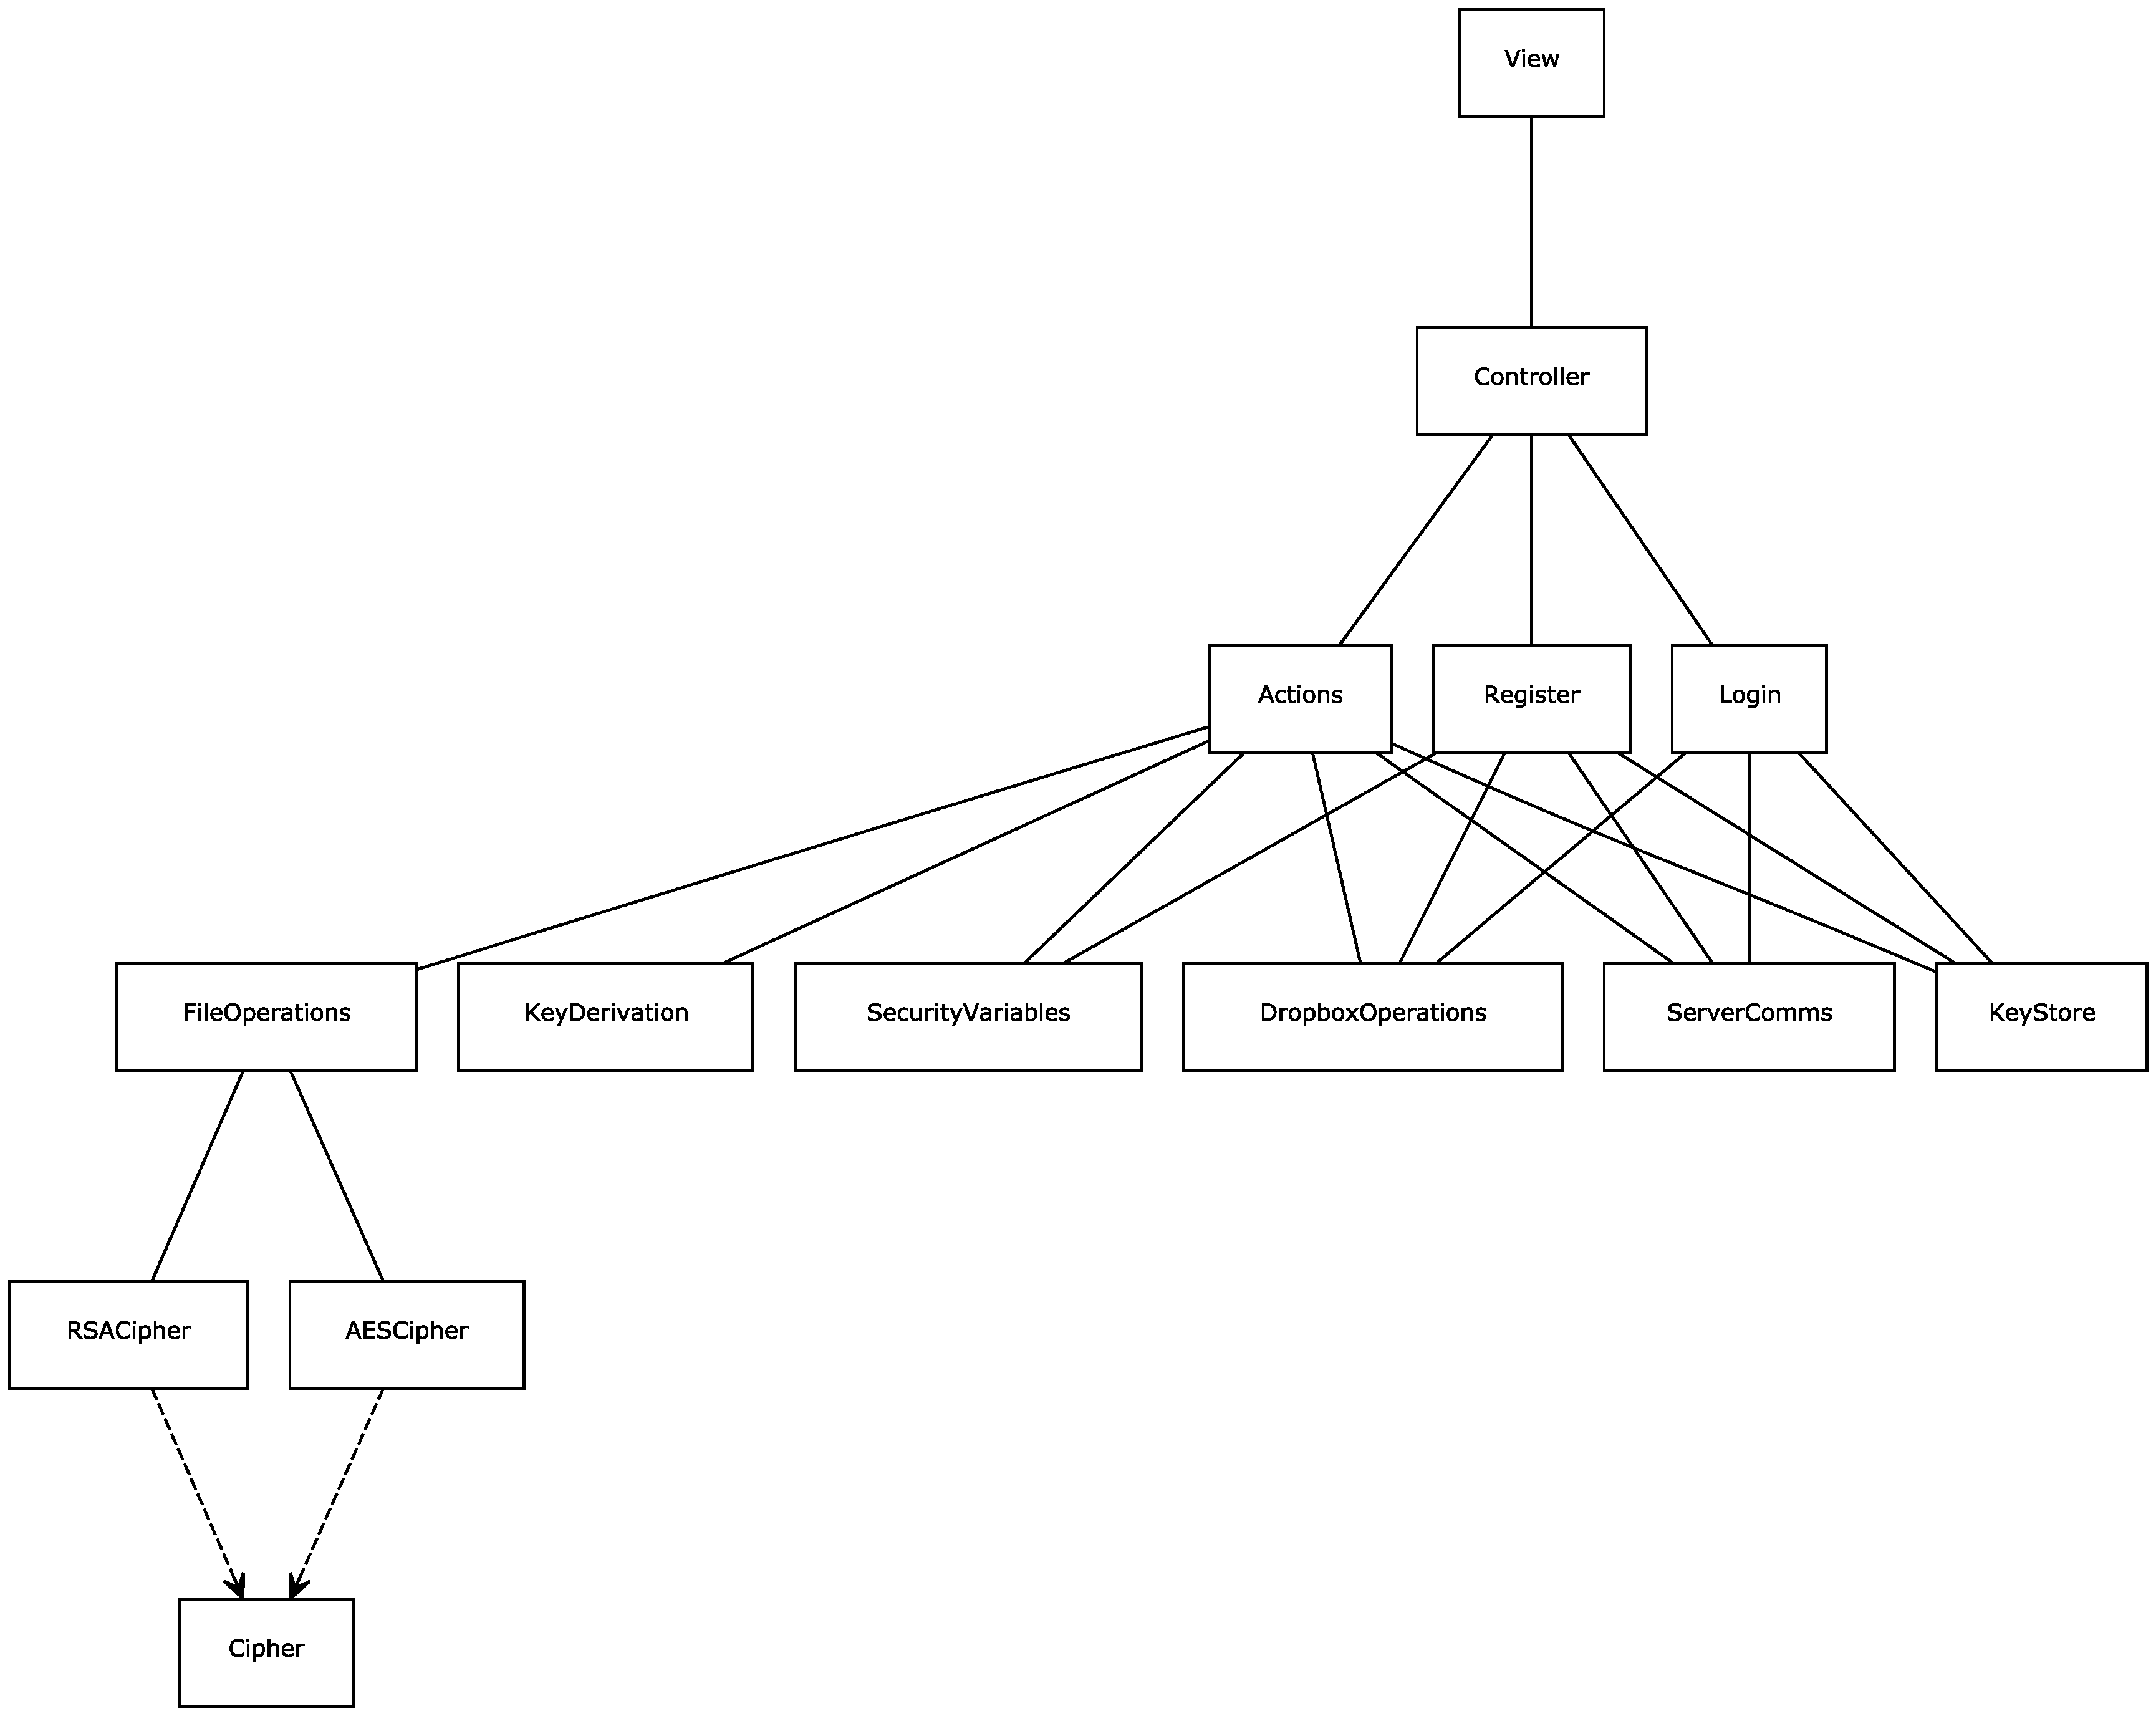
\includegraphics[height=5.0in,width=8in,angle=0]{client-classDiagram.pdf}}
\caption{Reduced class diagram for the client}
\label{fig:reducedClientClass}
\end{figure}

\subsubsection{Server}

\paragraph*{CentralAuthority} - This class mirrors the \textit{Actions} class in client. The class blocks until it receives a decision on which action the client wishes to perform. The class then communicates with the client for information and calls functions necessary to complete the request.
\paragraph*{UserOperations} - Acts as interface between the user logic and the table in the database containing user information.

\paragraph*{ServerDropboxOperations} - This class performs operations on a user's Dropbox which would be too unwieldly to perform client side. These include transferring files from one user to another and removing files when a user is revoked. These are difficult to perform on the client side as the actions are invoked by users which are not online at the time. Performing them safely on the client side would involve using database storage.



\subsection{Security}
When building a platform for users to control access to a resource, it is of upmost importance to ensure that this can not be circumvented by malicious users. Here we shall discuss some potential issues and how attempts were made to address them.
\subsubsection{Dropbox tampering}
Choosing to use Dropbox as the method to share files does not come free of security implications. One potential issue is the fact that it is entirely possible for a user to manipulate the folder in which the files for this application is stored outside of our application. The manipulation that could be can be divided into two categories. That is, manipulation of the folder containing their own uploaded files and manipulations of a folder containing files that their friend has shared with them. We shall address the former first. The potential manipulations that can be performed are:
\begin{itemize}
	\item Add a file to the folder containing their own uploads
	\item Remove a file in the folder containing their own uploads
	\item Edit a file in the folder containing their own uploads
\end{itemize}
For the manipulation in which a file is added to the folder containing a user's own uploads, the query to the server for file information will result in nothing being returned. We have options in how to deal with this. We could alert the user of the change and request information in order to handle the file, process the file as normal and treat it as regular upload. We could also simply ignore it. For now the file is simply ignored.
\newline \indent Removing a file from the user's own upload folder can be addressed in one of two ways, if the file has been shared we could replace the file in the user's uploads by copying it from one of their friends and then continue as normal. An alternative is to treat it as regular deletion and remove the file information from the database and remove it where it has been shared. Lastly, we could simply ignore it, however this results in the user losing control of the file and the friends with which they have shared it with can keep it and update it for as long as they like.
\newline \indent Manipulations in which a file is edited can be considered as a removal (of the file un-edited) and an addition (of the newly edited file) and can be treated as such.
\newline
\newline \indent The tampering of the folders of friend's shared files is a far more pressing security matter than that of tampering of user's own files. Here we shall discuss some potential issues. These issues are:
\begin{itemize}
	\item Create a folder for a user of which they have access at no level.
	\item Add a file to a folder containing a friend's uploads
	\item Remove a file in a folder containing a friend's uploads
	\item Edit a file in a folder containing a friend's uploads
\end{itemize}
Creating a folder for a user of which they have access at no level can only have the reaction of the being ignored.
\newline \indent When a user adds a file to a folder containing a friend's uploads our only safe option is to ignore it. To do this we must contact the server to verify the integrity of each file. Whether the file added is an encrypted file they do not have access to is not significant as they do not possess the key to decrypt it and the server can not be tricked into providing it as it does not possess any client keys.
\newline \indent Removing a file from a folder containing a friend's uploads can be ignored, meaning that they will no longer has access to the file, at least until someone updates it. Or we could simply replace the file by copying the owner's current version of the file.

\section{Testing}




\section{Evaluation}

\subsection{User stories}

\subsection{What I would have done differently}
Replacing keys automatically after a set period of time. (ie. they expire)
\\ Implement adjustable lower bounds as per Jason Crampton's algorithm.
\\ Employ a more lazy key revocation scheme.

\section{Conclusion}

\subsection{Achievements}

\subsection{Future work}

\begin{thebibliography}{10}

\bibitem{appliedCryptoBook}
Bruce Schneier, \emph{``Applied Cryptography: Protocols, Algorithms, and Source Code in C"}, 1995.

\bibitem{newCryptoDirections}
Diffie and Hellman, \emph{``New Directions in Cryptography"},
IEEE Transactions on Information Theory, Vol. IT-22, No.6, 1976.

\bibitem{classicalCryptoBook}
S Vaudenay, \emph{``A Classical Introduction to Cryptography: Applications for Communications Security"}, 2005.

\bibitem{blockCiphers}
A. Menezes, P. van Oorschot and S. Vanstone, \emph{``Handbook of Applied Cryptography"}, Chapter 7, CRC Press, 1996.

\bibitem{accessControlPrinciples}
Sandhu and Samarati, \emph{``Access Control: Princples and Practice"},
IEEE Communications Magazine, September 1994.

\bibitem{bittorrent}
Fu, Kamara and Kohno, \emph{``Key Regression$\colon$ Enabling Efficient Key Distribution for Secure Distributed Storage"}, 2005.

\bibitem{mainPaper}
Jason Crampton, \emph{``Practical and Efficient Cryptographic Enforcement of Interval-Based
Access Control Policies"}, Royal Holloway, University of London, 2011.

\bibitem{atallahGeo}
Atallah et al, \emph{``Efficient Techniques for Realizing Geo-spatial Access Control"},  Purdue University, 2007.

\bibitem{atallah2005}
Atallah et al, \emph{``Dynamic and Efficient Key Management for Access Hierarchies"}, Purdue University, 2005 (revised 2009).

\bibitem{blanton2007}
Blanton, \emph{``Key Management in Hierarchical Access Control"}, Ph.D. Thesis, Purdue University, 2007.

\bibitem{lazyEncryption}
Jason Crampton, \emph{``Cryptographically-Enforced Hierarchical
Access Control with Multiple Keys"}, Information Security Group, Royal Holloway, University of London, 2009.

\bibitem{largeLeaf}
JW Lo, MS Hwang and CH Liu, \emph{``An Efficient Key Assignment Scheme for Access Control in a Large Leaf Class Hierarchy}, Information Sciences, 2011.

\bibitem{ecc1}
AK Das, NR Paul and L Tripathy, \emph{``Cryptanalysis and Improvement of an Access Control in User Hierarchy Based on Elliptic Curve Cryptosystem"}, Information Sciences, 2012.

\bibitem{ecc2}
YL Lin, CL Hsu, \emph{``Secure key management scheme for dynamic hierarchical access control based on ECC"}, Journal of Systems and Software, 2011.

\bibitem{delete}
Radia Perlman, \emph{``File System Design with Assured Delete"}, Sun Microsystems, 2005.

\bibitem{pyCrypto}
Dwayne C. Litzenberger, \emph{``PyCrypto - The Python Cryptography Toolkit"},
\\ Available at: \texttt{https://www.dlitz.net/software/pycrypto/}.

\bibitem{javaJCA}
\emph{``Java\texttrademark Cryptography Architecture (JCA) Reference Guide"},
\\ Available at: \texttt{http://docs.oracle.com/javase/6/docs/technotes/guides/security/crypto/CryptoSpec.html}.

\bibitem{bouncyCastle}
\emph{``The Legion of the Bouncy Castle"},
\\ Available at: \texttt{http://www.bouncycastle.org/java.html}.

\bibitem{gnuCrypto}
\emph{``The GNU Crypto project"},
\\ Available at: \texttt{https://www.gnu.org/software/gnu-crypto/\#introduction}.

\bibitem{rubyOpenSSL}
\emph{"openssl: Ruby Standard Library Documentation"},
\\ Available at: \texttt{http://www.ruby-doc.org/stdlib-1.9.3/libdoc/openssl/rdoc/index.html}.

\bibitem{keyczar}
\emph{"Keyczar"}, Available at: \texttt{http://www.keyczar.org/}.

\bibitem{aesFIPSApproved}
Randall J. Easter and Carolyn French, \emph{Approved Security Functions
for FIPS PUB 140-2}, May 30 2012,
\\ Available at: \texttt{http://csrc.nist.gov/publications/fips/fips140-2/fips1402annexa.pdf}.

\bibitem{aesModes}
NIST, \emph{Recommendation for Block Cipher Modes of Operation}, 2001 Edition
\\ Available at: \texttt{http://csrc.nist.gov/publications/nistpubs/800-38a/sp800-38a.pdf}.

\bibitem{oraclePadding}
Juliano Rizzo and Thai Duong, \emph{Practical Padding Oracle Attacks}, May 25th 2010,
\\ Available at: \texttt{\url{http://static.usenix.org/events/woot10/tech/full_papers/Rizzo.pdf}}.


\bibitem{nistKeys}
Elaine Barker, William Barker, William Burr, William Polk, and Miles Smid, \emph{NIST Special Publication 800-57}, Recommendation for Key Management – Part 1: General (Revision 3), July
2012,
\\ Available at: \texttt{\url{http://csrc.nist.gov/publications/nistpubs/800-57/sp800-57_part1_rev3_general.pdf}}

\bibitem{announcingAES}
FIPS, \emph{Announcing the ADVANCED ENCRYPTION STANDARD (AES)}, November 26, 2001,
\\ Available at:
\texttt{http://csrc.nist.gov/publications/fips/fips197/fips-197.pdf}.

\bibitem{nistPassword}
Meltem Sönmez Turan, Elaine Barker, William Burr, and Lily Chen, \emph{NIST Special Publication 800-132}, Recommendation for Password-Based Key Derivation, Part 1: Storage Applications, December 2010,
\\ Available at: \texttt{http://csrc.nist.gov/publications/nistpubs/800-132/nist-sp800-132.pdf}.

\bibitem{oaepAttack}
James Manger, \emph{A Chosen Ciphertext Attack on RSA Optimal Asymmetric Encryption Padding (OAEP) as Standardized in PKCS \#1 v2.0}, 2001.

\bibitem{bcryptPaper}
Niels Provos and David Mazières, \emph{A Future-Adaptable Password Scheme}, 1999 USENIX Annual Technical Conference, June 6–11 1999,
\\ Available at: \texttt{http://static.usenix.org/event/usenix99/provos/provos.pdf}. 

\bibitem{dropboxPublicFolder}
Dropbox API Team, \emph{``New sharing model will replace Public folder"},  15th June 2012,
\\ Available at: \texttt{https://www.dropbox.com/developers/blog/19}.

\end{thebibliography}

\end{document}


